\documentclass[12pt,a4paper]{article}
\usepackage[utf8]{inputenc}
\usepackage{amsmath}
\usepackage{amsfonts}
\usepackage{amssymb}
\usepackage{graphicx}
\usepackage{float}
\usepackage[font=small,labelfont=bf]{caption}
\usepackage{tabularx}
\usepackage{siunitx}
\usepackage[LGRgreek]{mathastext}
\usepackage{cancel}
\usepackage{ulem}
\usepackage{comment}

\usepackage{listings}
\usepackage{xcolor}

\definecolor{codegreen}{rgb}{0,0.6,0}
\definecolor{codegray}{rgb}{0.5,0.5,0.5}
\definecolor{codepurple}{rgb}{0.58,0,0.82}
\definecolor{backcolour}{rgb}{0.95,0.95,0.92}

\lstdefinestyle{mystyle}{
    backgroundcolor=\color{backcolour},   
    commentstyle=\color{codegreen},
    keywordstyle=\color{magenta},
    numberstyle=\tiny\color{codegray},
    stringstyle=\color{codepurple},
    basicstyle=\ttfamily\footnotesize,
    breakatwhitespace=false,         
    breaklines=true,                 
    captionpos=b,                    
    keepspaces=true,                 
    numbers=left,                    
    numbersep=5pt,                  
    showspaces=false,                
    showstringspaces=false,
    showtabs=false,                  
    tabsize=2
}

\lstset{style=mystyle}



\newcommand{\stkout}[1]{\ifmmode\text{\sout{\ensuremath{#1}}}\else\sout{#1}\fi}
%police et mise en page (marges) du document
\usepackage[T1]{fontenc}
\usepackage[top=2cm, bottom=2cm, left=2cm, right=2cm]{geometry}


\makeatletter
\newcommand\subsubsubsection{\@startsection{paragraph}{4}{\z@}{-2.5ex\@plus -1ex \@minus -.25ex}{1.25ex \@plus .25ex}{\normalfont\normalsize\bfseries}}
\newcommand\subsubsubsubsection{\@startsection{subparagraph}{5}{\z@}{-2.5ex\@plus -1ex \@minus -.25ex}{1.25ex \@plus .25ex}{\normalfont\normalsize\bfseries}}
\makeatother


\begin{document}


%-------debut titre
\begin{titlepage}
\begin{minipage}[c]{.46\linewidth}
     \begin{center}
         %-------------------LOGO--------------------
         \includegraphics[width=6cm]{../../../tele.jpg}   
         
         \end{center}
   \end{minipage} \hfill
   \begin{minipage}[c]{.46\linewidth}
    \begin{center}
    	%-------------------LOGO--------------------
       \includegraphics[width=5cm]{../../../le2p.png}   
        \end{center}
 \end{minipage}
\newcommand{\HRule}{\rule{\linewidth}{0.5mm}}
\center
\textsc{\LARGE} \\[3cm]

\HRule \\[0.4cm]
{ \huge \bfseries Rapport de stage\\ [0.15cm] }
\HRule \\[1cm]

\textbf{ Mise à niveau d'un instrument de mesure du rayonnement diffus par arc d’ombrage}\\[1cm]
\textbf{ Du 06 avril 2021 au 04 juin 2021}\\[8cm]
%---------------------image illustration----------------
%\includegraphics[scale=1]{image/big.png} \\ [2cm]
\begin{tabular}{lll}
   \sf Stagiare: &\sf Responsable Pédagogique: &\sf Tutrice de stage : \\
  \sf Alexandre PARASSOURAMIN &\sf Mme Béatrice MOREL &\sf Mme Béatrice MOREL \\
   \sf Master 1 énergie& &\\
  \sf n$^\circ$~étudiant : 35003702& & \\
\end{tabular}




\end{titlepage}
%-----Fin titre
\newpage
\thispagestyle{empty}

\section*{Remerciements}
\sf
Je tiens tout d'abord à remercier ma tutrice de stage Mme Béatrice MOREL.\\
~\\
Je tiens ensuite à remercier tout particulièrement M. Jeanty PATRICK, M. Mathieu DELSAUT et M. Christian BROUAT pour l'accompagnement durant le stage.\\
~\\
Je tiens aussi à remercier M. Yannis HOARAU pour l'utilisation de l'imprimante 3D.
 
 
~


\newpage







\thispagestyle{empty}
\renewcommand{\contentsname}{Sommaire}
\tableofcontents
\newpage

\newpage


\begin{flushleft}


\sf
\section*{Introduction}
\addcontentsline{toc}{section}{\protect\numberline{}Introduction}%
\setcounter{page}{3}

Dans le cadre de mon master 1 j'ai dû réaliser un stage de huit semaines, le stage s'est déroulé au sein du laboratoire LE2P de l'université de la Réunion.\\
~\\
Le stage avait pour objectif le montage d'un pyranomètre à arc d'ombrage cm121, l'élaboration d'un calendrier de maintenance pour le cm121, la mise en place d'un protocole permettant le réglage la position Nord-sud, le développement des programmes sous python permettant l'analyse statistique des mesures de rayonnement diffus. Le stage vise aussi à répondre à deux questions, la premières est de savoir si les mesures du cm121 sont plus proches du spn1 ou du tracker, et finalement de savoir si l'installation d'une ventilation à un impact sur les mesures du CM121.
 

\section{Environnement}



Le laboratoire LE2P, a été créé en 2006,  il est membre de l’Observatoire des Milieux Naturels et des Changements Globaux au sein de la Faculté des Sciences et Technologies de L’Université de La Réunion. Le laboratoire comporte trois opérations scientifiques qui sont au cœur des projets menés par la Région Réunion.\\
~\\
L'opération scientifique gisement Solaire : variabilité à La Réunion et en zone tropicale, métrologie et modélisation  vise à offrir une documentation sur la variabilité du rayonnement solaire.\\
~\\
L'opération scientifique optimisation-contrôle et stockage de l'énergie, se penche sur la conception et le design d’une Pile A Combustible réversible ainsi que la modélisation et le contrôle d’une Pile A Combustible de type PEMFC.\\ 
~\\
L'opération scientifique réseau interconnecté et transport de l'énergie étudie l’évolution énergétique d'un réseau, le développement de topologies et de protocoles de routage à faible coût énergétique et la récupération d’énergie RF.



\section{Les travaux effectués et les apports du stage}



\subsection{Montage du CM121C}

Le CM121 comportes cinq parties, la base, le pilier, la barre transversale, la barre coulissante et le support pour pyranomètre. Le montage consiste juste à assembler chaque partie à l'aide des boulons fournis.

\begin{figure}[H]
\centering
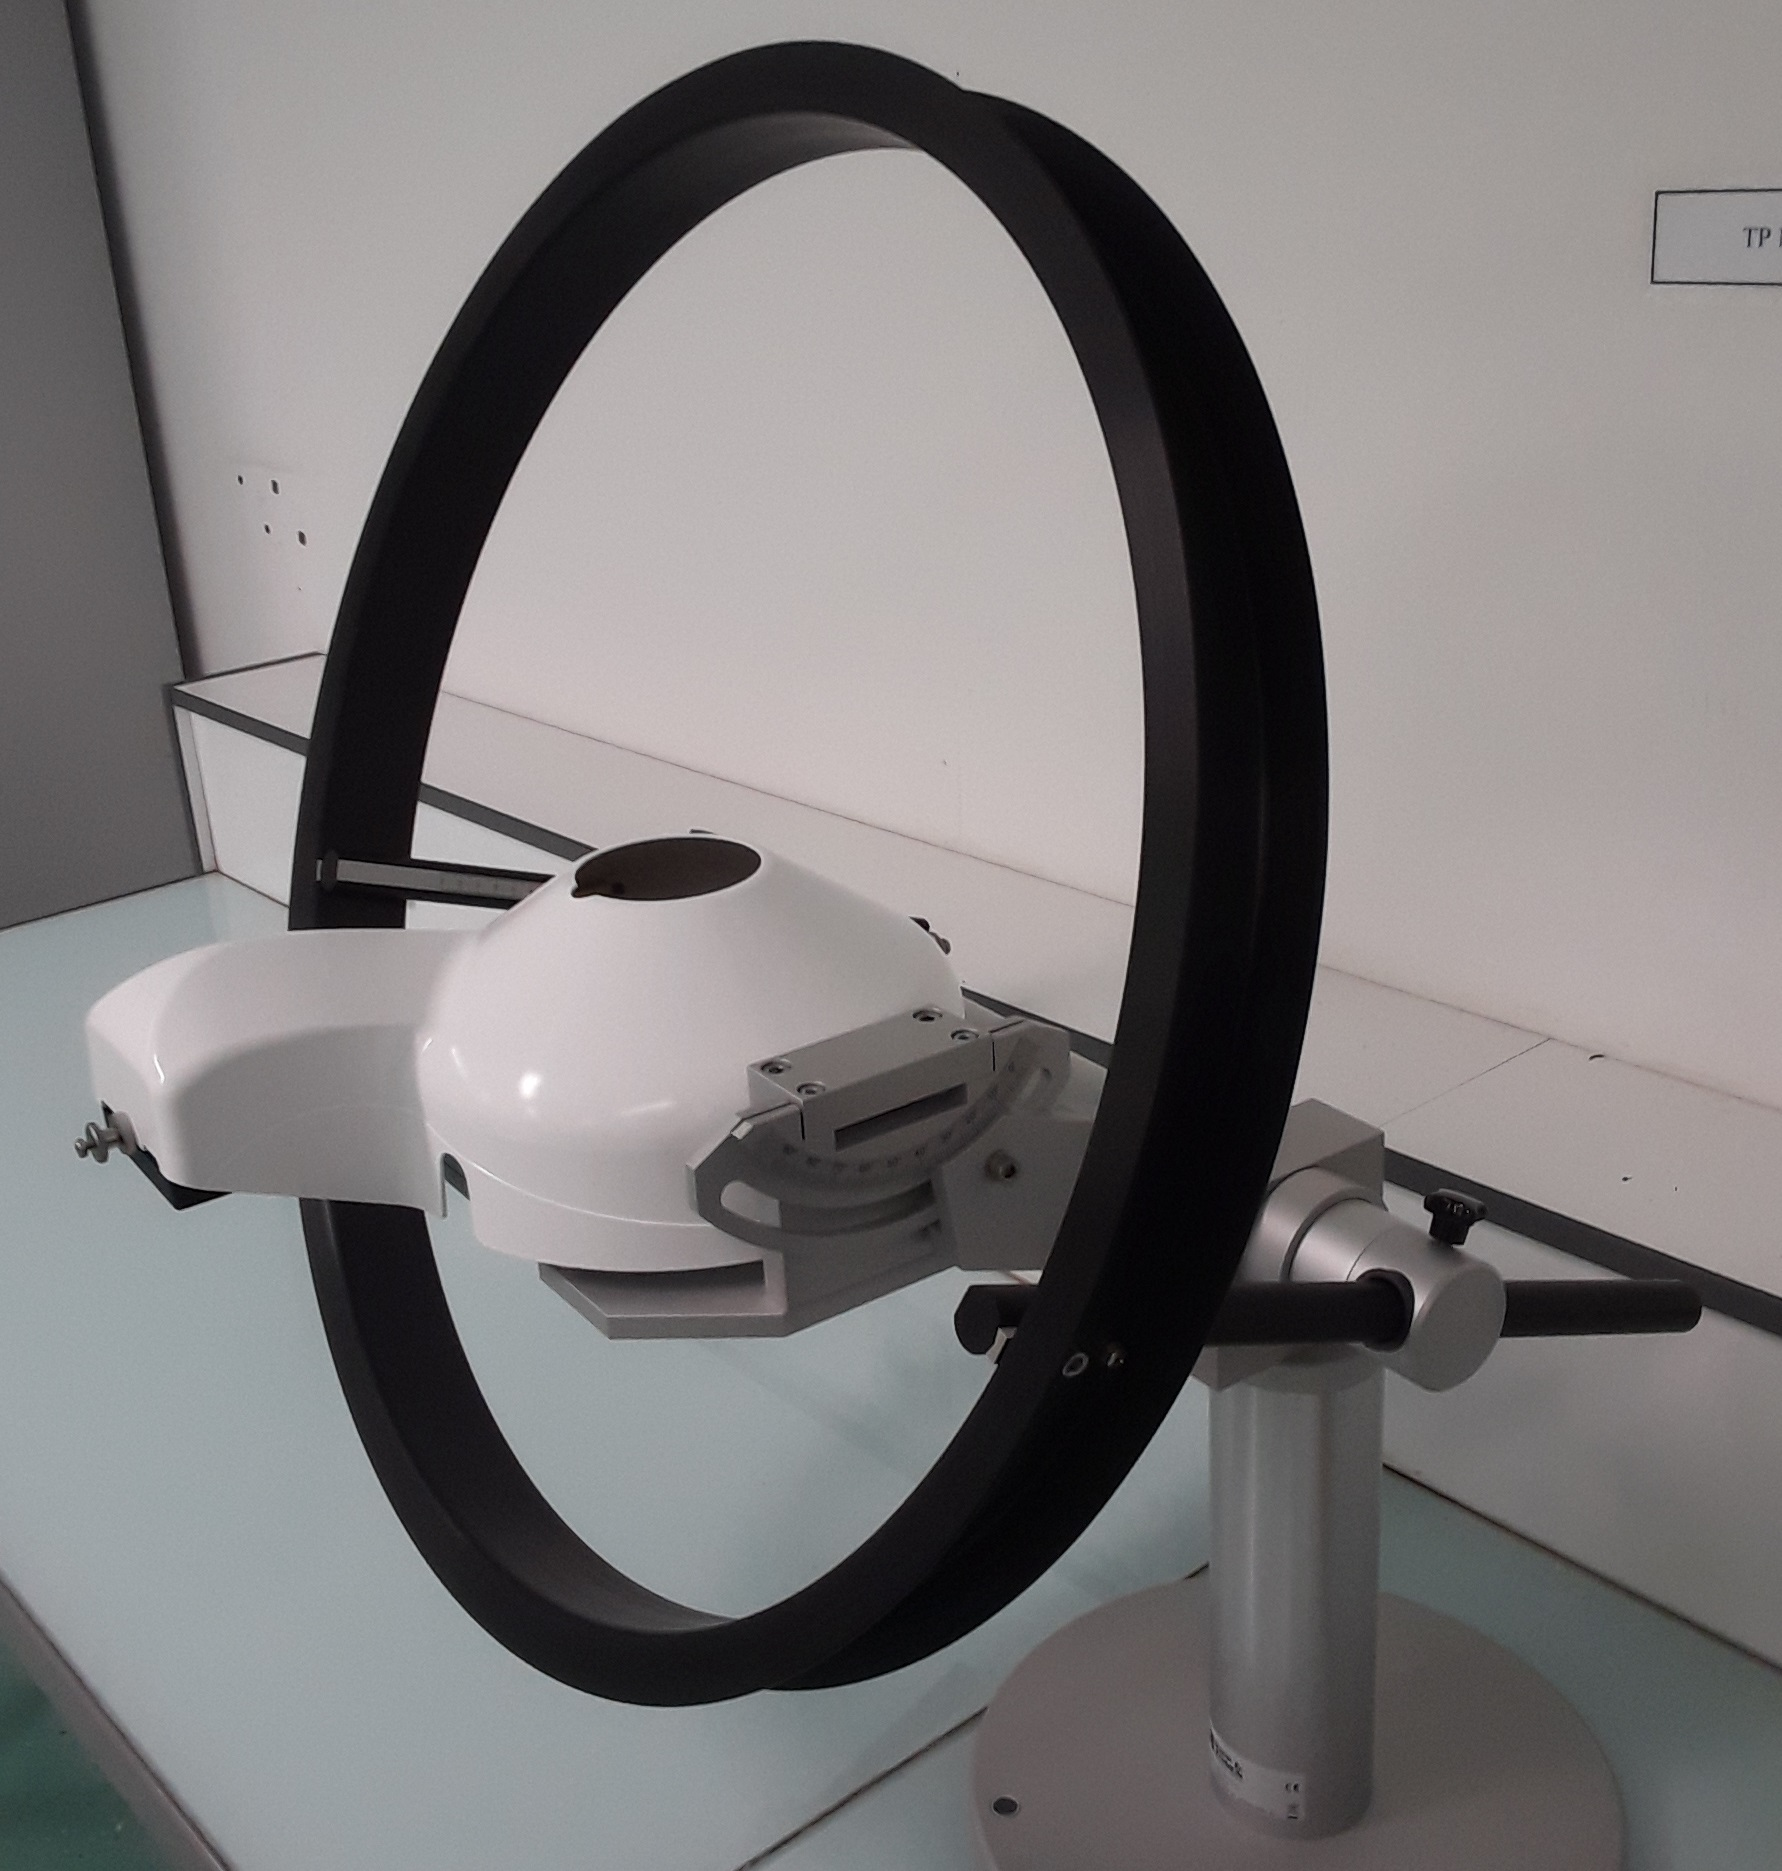
\includegraphics[width=10cm]{image/montage/1.jpg} 
\caption{cm121}
\end{figure}


La première étape pour le positionnement du cm121 consiste à s'assurer que sa base est plane, pour se faire la base comporte 3 boulons permettant à l'aide d'un niveau à bulle de mettre la base à l'horizontale.. 

\begin{figure}[H]
\centering
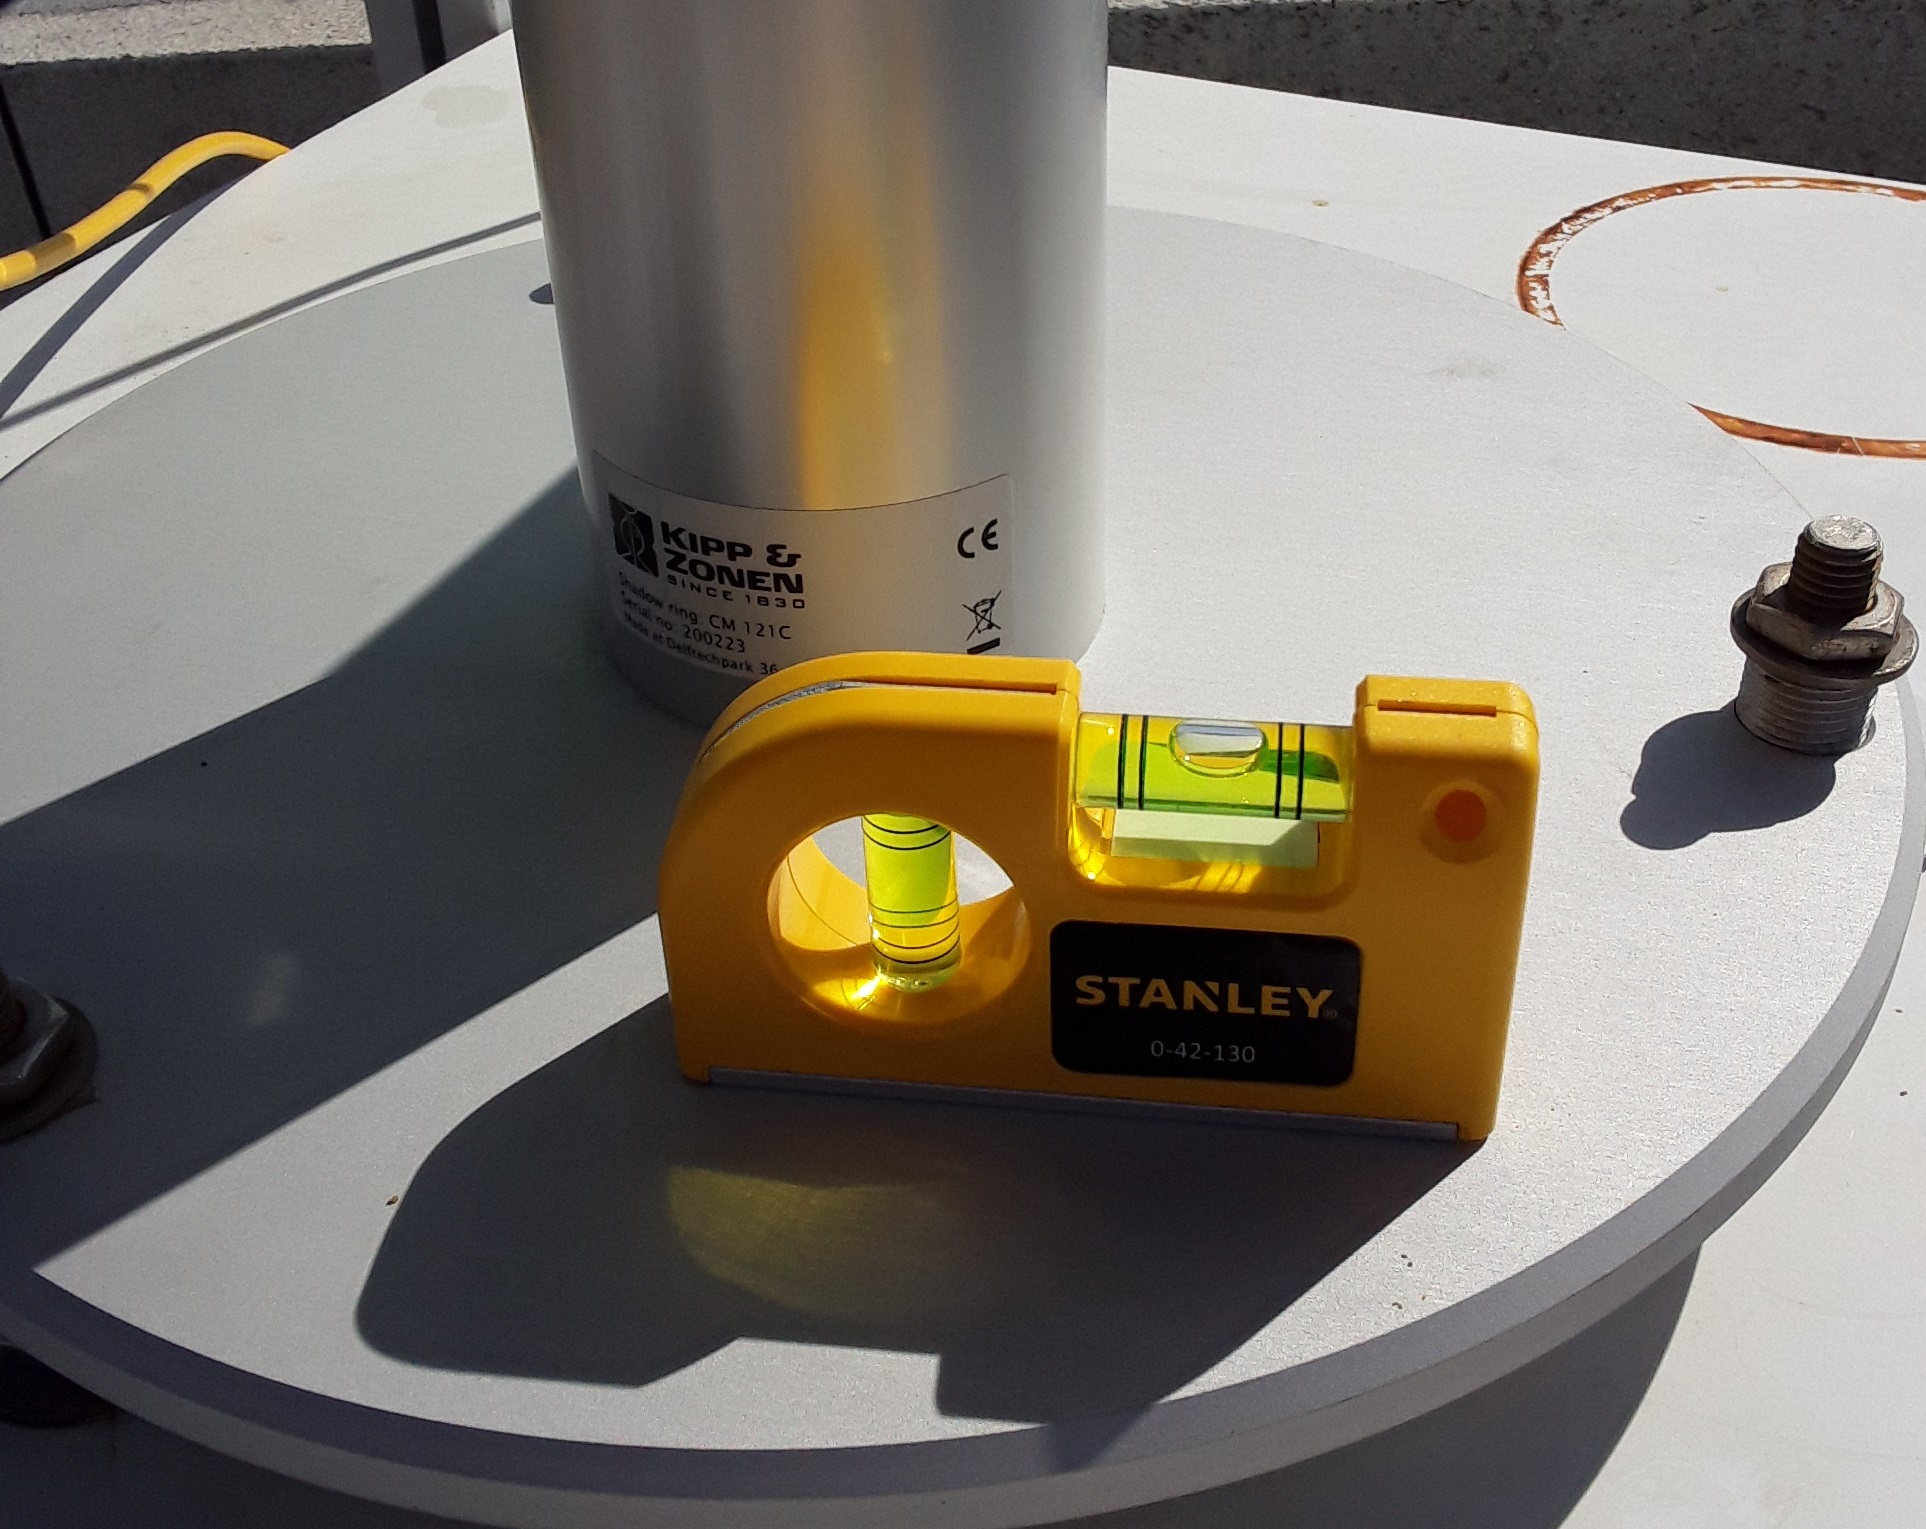
\includegraphics[width=10cm]{image/montage/2.jpg} 
\caption{Base horizontal}
\end{figure}


La barre coulissante doit être parallèle à l'axe polaire, pour se faire l'angle entre l'horizon et la barre doit être égal à la latitude du site, pour l'Université de la Réunion cela implique un angle de -20.9$^\circ$. L'angle est réglé grace à une application mobile qui offre une précision acceptable, le réglage pouvant se faire à 1-4 degrés prêts selon la datasheet.

\begin{figure}[H]
\centering
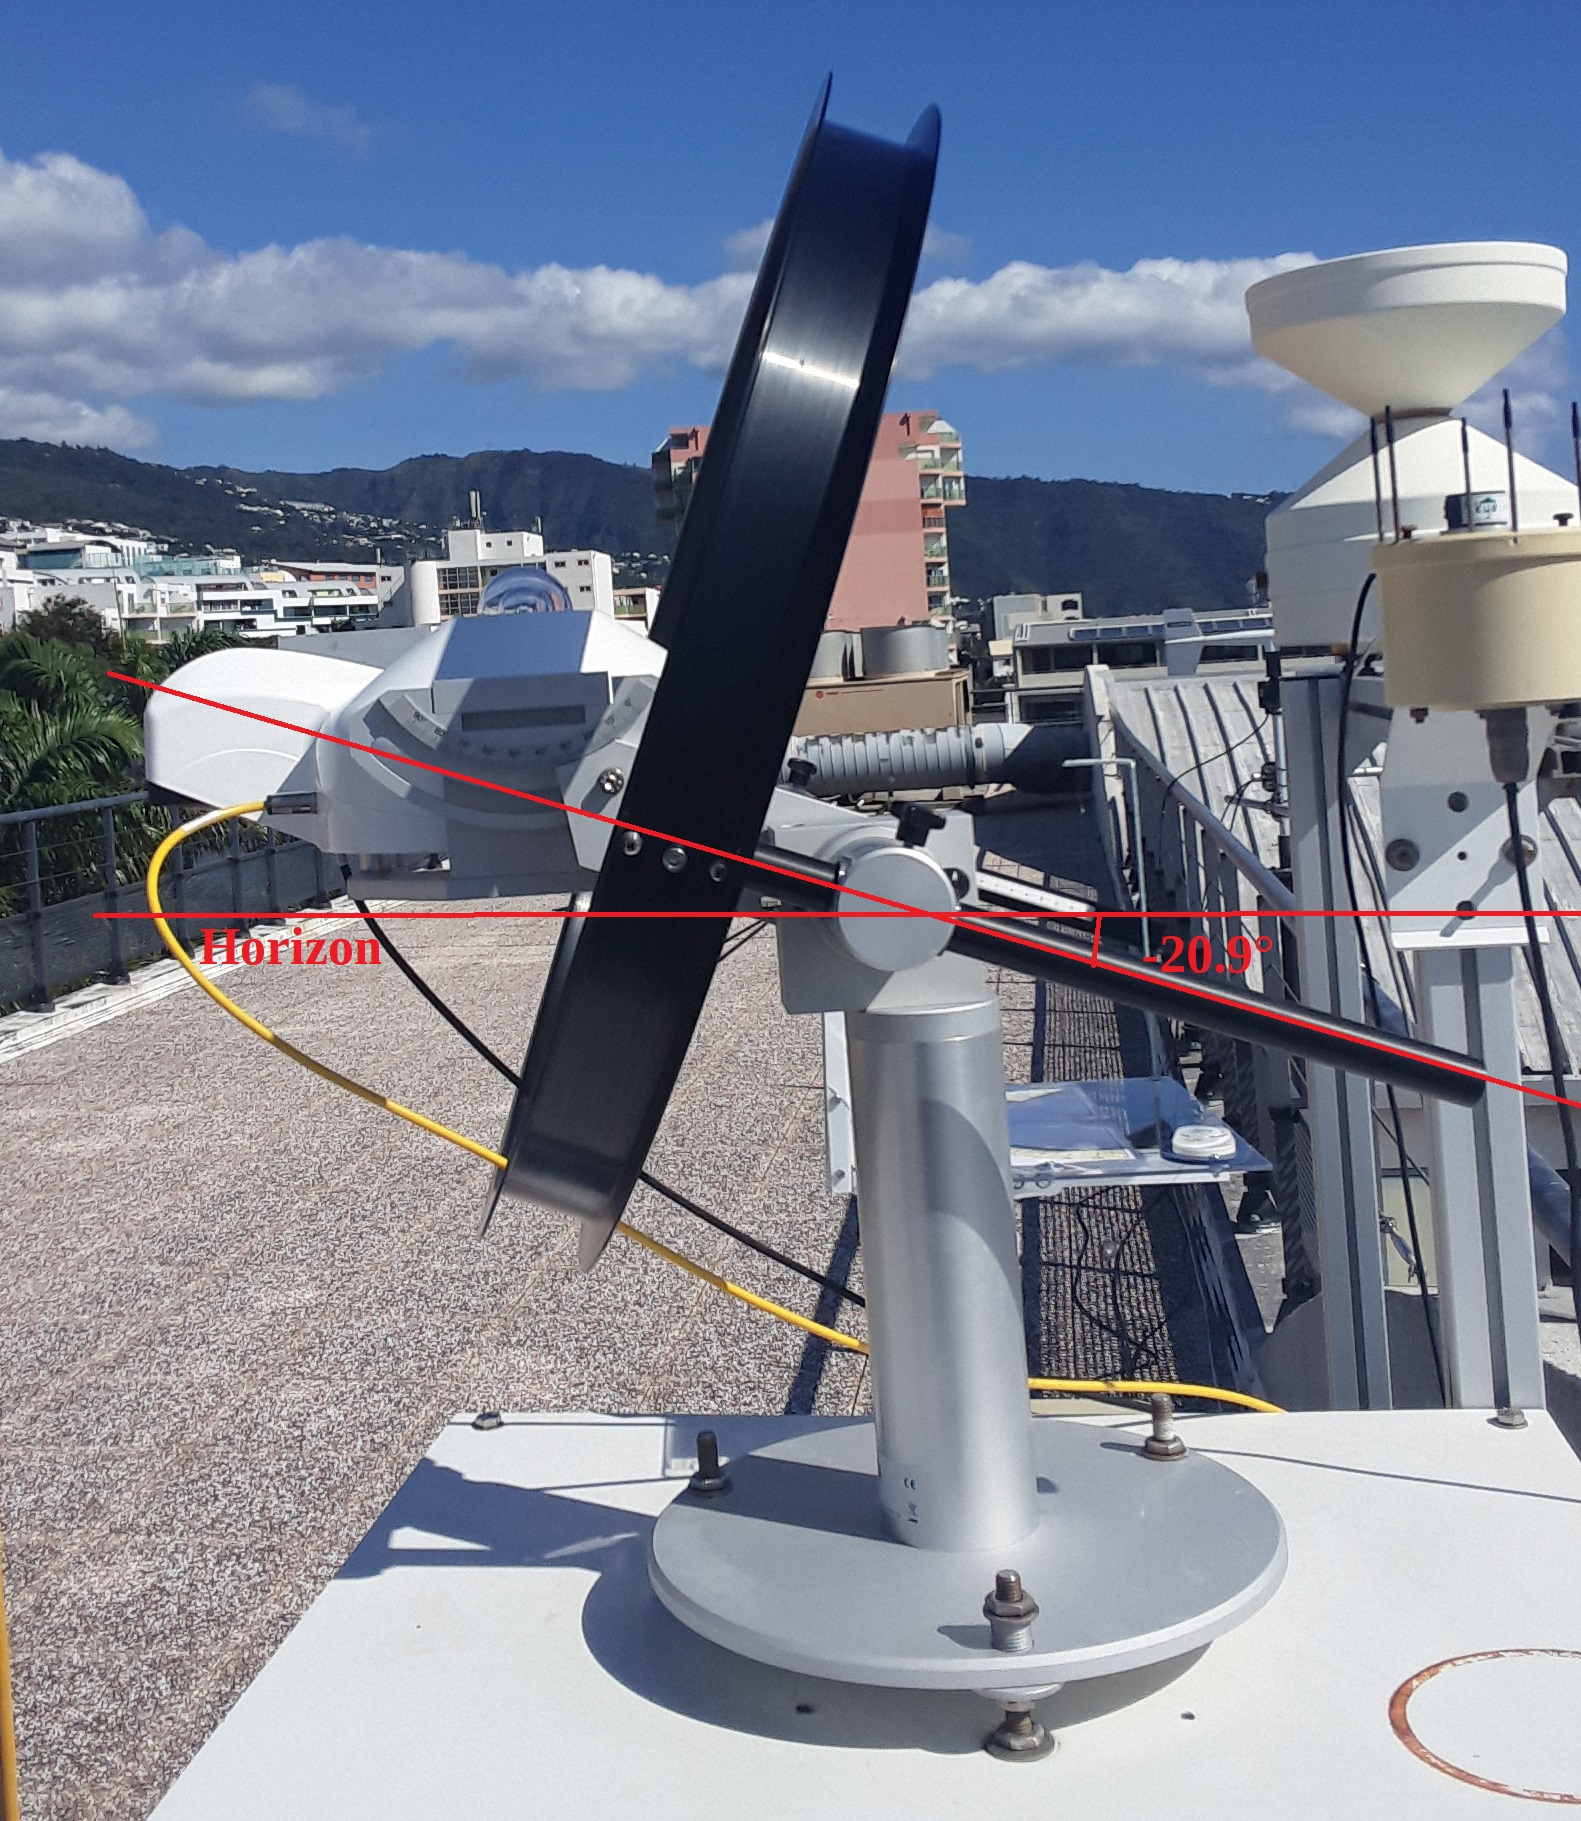
\includegraphics[width=10cm]{image/montage/3.jpg} 
\caption{Axe polaire}
\end{figure}


Le pyranomètre est installé sur son socle. Une fois effectuer la ventilation est installé est raccordé en 12 volts. La ventilation permet de garder le pyranomètre à température constante, permettant ainsi de faire l'acquisition des mesures dans les mêmes conditions de températures toute l'année.

\begin{figure}[H]
\centering
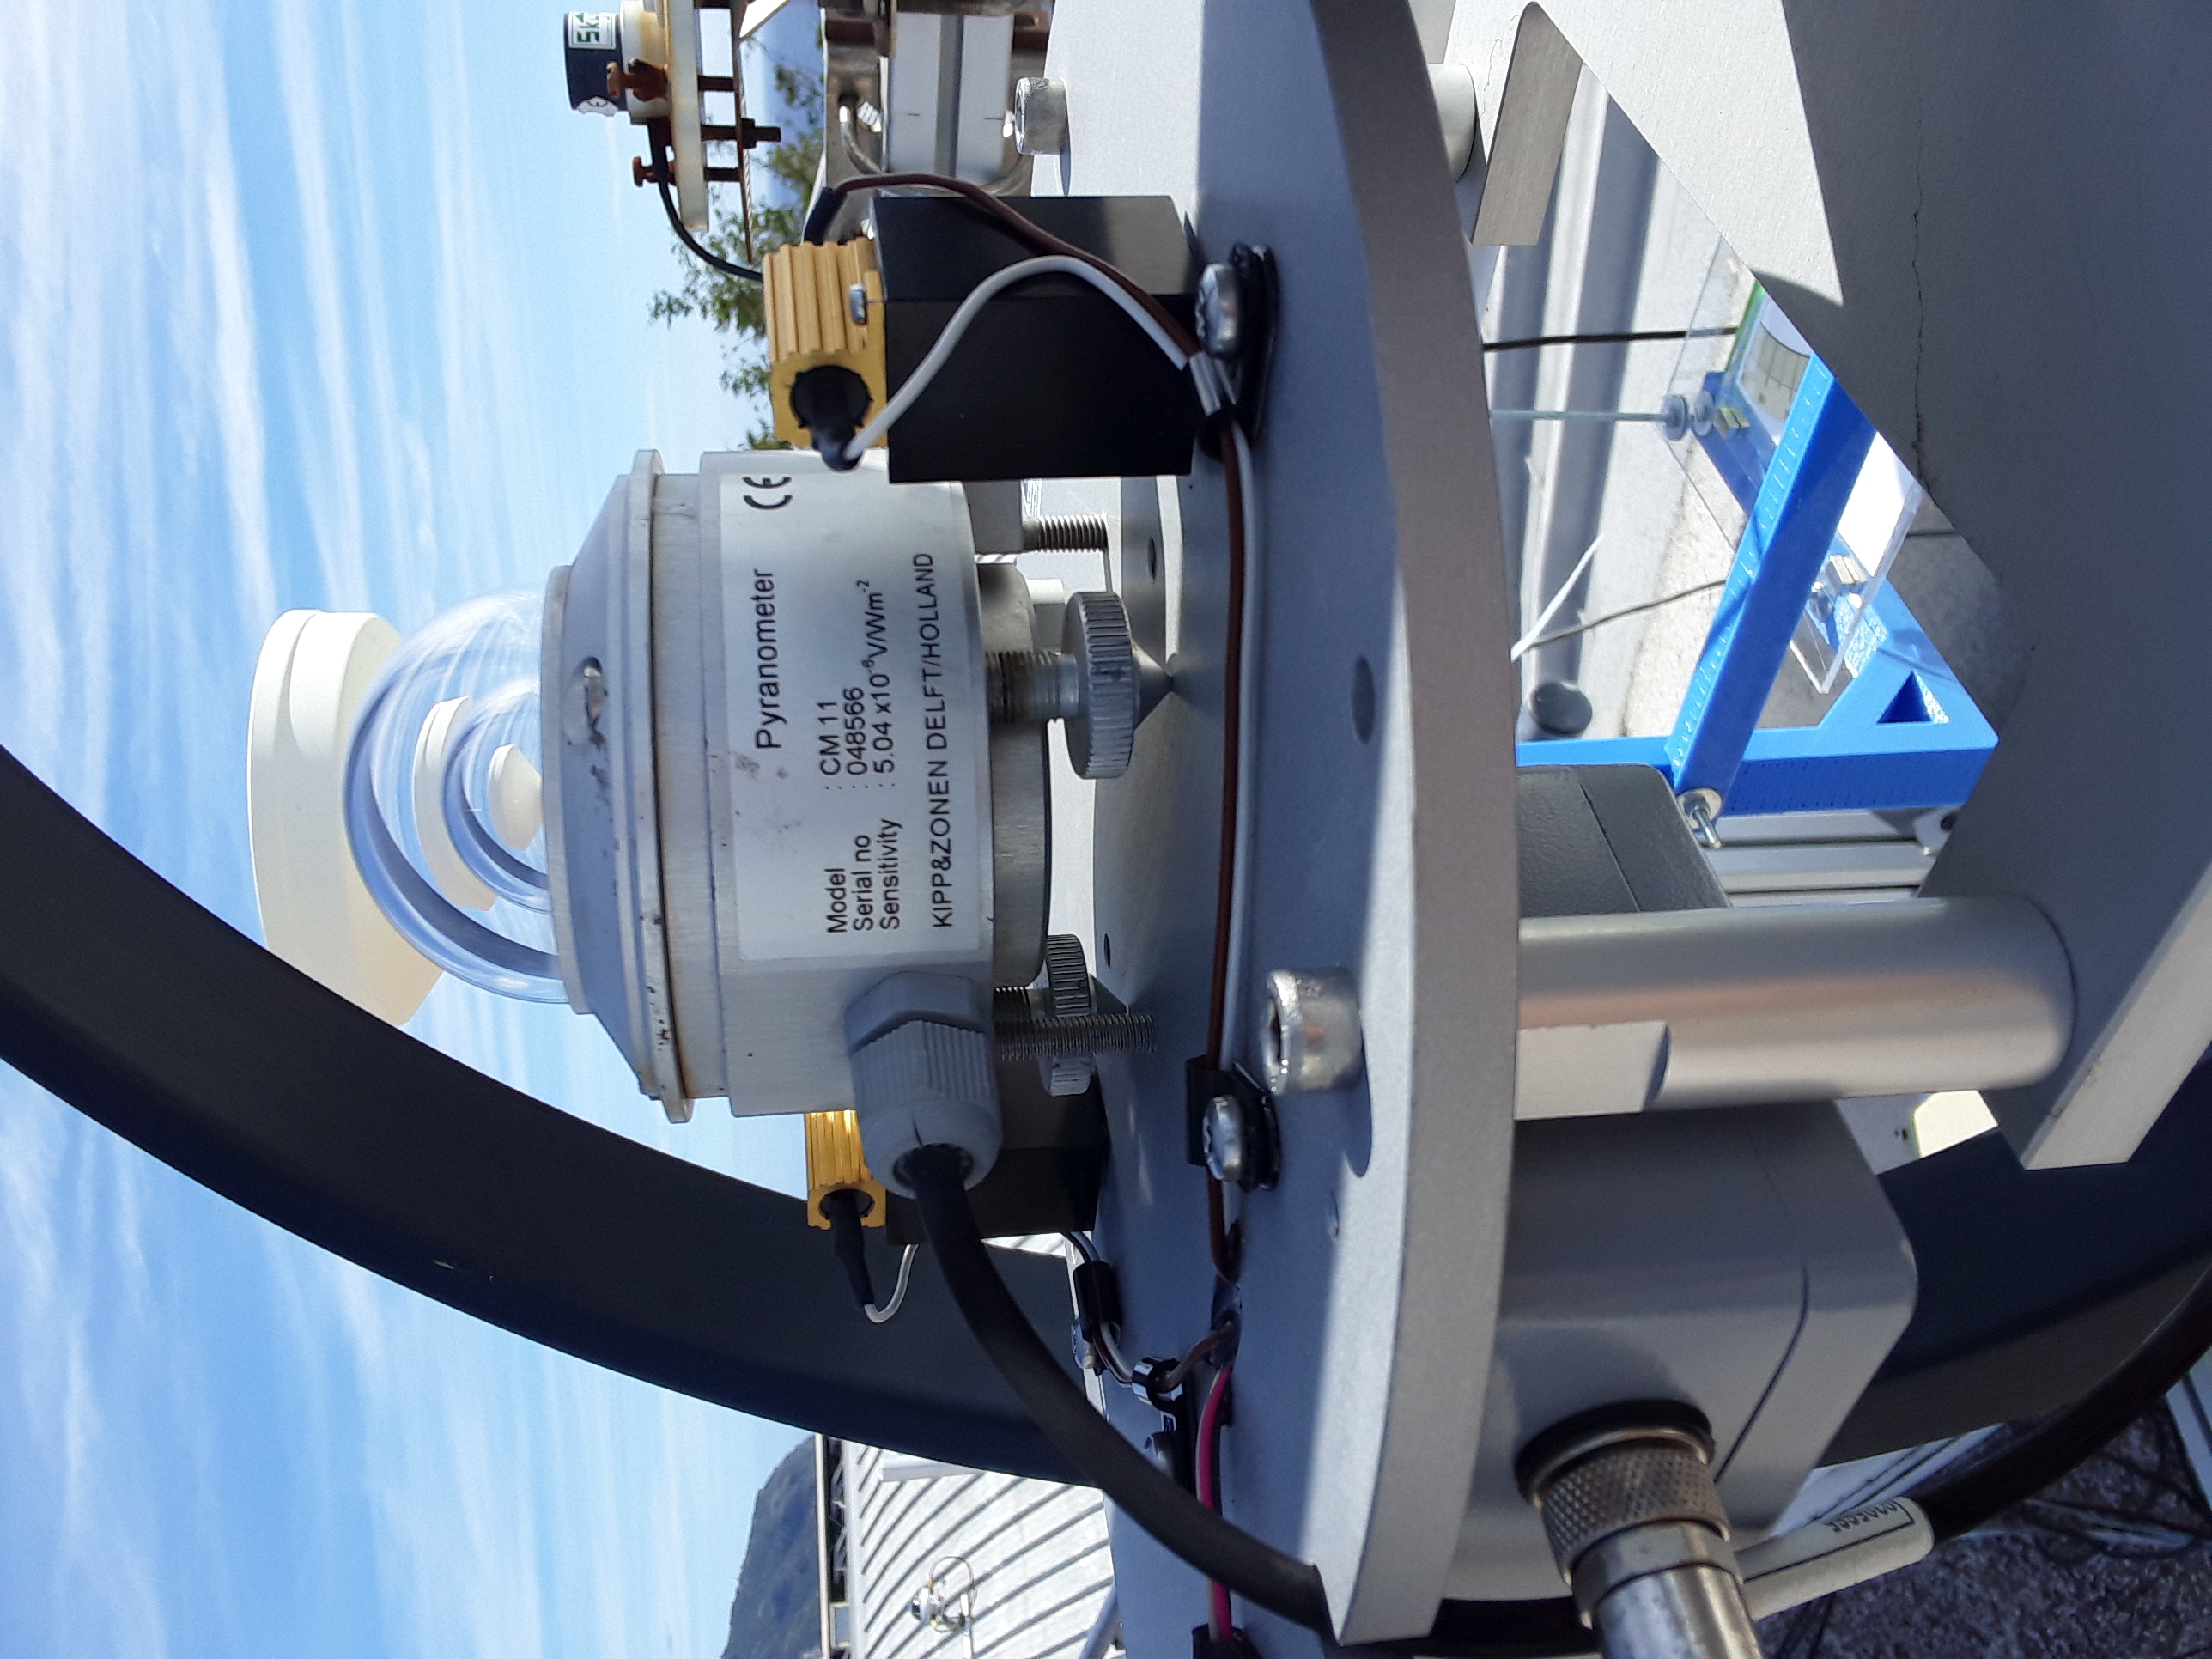
\includegraphics[width=10cm, angle=-90]{image/montage/4.jpg} 
\caption{Installation pyranomètre}
\end{figure}


L'étape la plus importante et le réglage de la position nord-sud, un mauvais réglage nord-sud peuvent entrainer des données aberrantes, du fait que le capteur est susceptible de recevoir du rayonnement global à certains moments de la journée. Une première approche pourrait consister à utiliser un compas magnétique mais la présence d'éléments ferreux donne une indication fausse du nord. La méthode retenue est l'utilisation d'une boussole solaire.\\
~~\\
Le principe de la boussole solaire est de projeter l'ombre du soleil sur une surface plane, sur cette surface plane se trouve un cadran gradué représentant l'azimut, en connaissant l'azimut du soleil et en reportant l'ombre sur le cadran nous obtenons la position nord-sud.\\

\subsubsection{Alignement nord-sud par pointage géographique}

Le premier alignement Nord-sud fut effectué par une boussole solaire totalement indépendante de l'arc d'ombrage, le but consiste à l'aide d'une feuille excel et de l'heure actuelle, de calculer l'azimut, de la reporter sur la boussole solaire en la faisant pivoter et de pointer un point géographique passant dans l'axe nord-sud de la boussole solaire. Une fois ce point géographique trouvé, nous effectuons la même démarche en reportant ce point dans l'axe de la barre coulissante.\\

Cette méthode donne de bons résultats, mais elle nous expose à des erreurs d'angle notamment lors du pointage du point géographique et le vent faisant bouger le fil, elle a aussi pour inconvénient une mise en place assez lourde avec l'obligation d'avoir un ordinateur portable sous la main.\\	

\begin{figure}[H]
\centering
\includegraphics[width=10cm, angle=-90]{image/montage/5.jpg} 
\caption{Boussole solaire}
\end{figure}

\begin{figure}[H]
\centering
\includegraphics[width=10cm]{image/montage/6.jpg} 
\caption{Point géographique}
\end{figure}

\subsubsection{Alignement nord-sud par boussole solaire fixe}   

Pour pallier les problèmes de la boussole solaire traditionnelle, il fit élaborer une boussole solaire fixe. Le but est de faciliter le réglage nord-sud, mais aussi de diminuer les erreurs d'angles de la boussole traditionnelle, pour se faire la boussole devra être fixée à la barre transversale du cm121.\\
~\\
Pour faciliter la maintenance le choix de la conception s'est porté sur l'impression 3D, la modélisation fut effectué sur le logiciel fusion 360 (figure *). La boussole comporte 4 parties imprimer en 3D (deux bases et deux longerons), une plaque de plexiglas permettant de placer notre cadran d'azimut et une tige filetée qui sert de support au fil.\\



Les quatre parties imprimées en 3D sont assemblées à l'aide de quatre boulons de 3*20mm.\\

\begin{figure}[H]
\centering
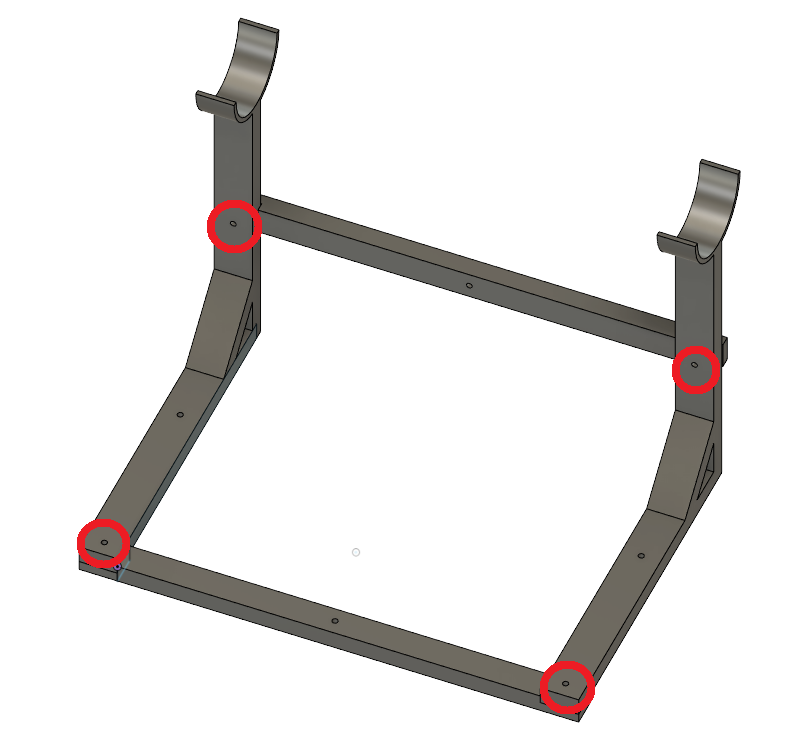
\includegraphics[width=12cm]{image/montage/boussole_solaire/2.png} 
\caption{Assemblage bases et longerons}
\end{figure}

Trois boulons de 3*30mm viennent se placer aux endroits prévus, ces boulons permettent de régler la plaque de plexiglas pour qu'elle soit horizontale. La plaque de plexiglas est coupé dans du plexiglas de 3 mm et les passages de boulon sont percé par une mèche de 3 mm. La plaque repose sur les trois boulons de 3*30mm.\\

\begin{figure}[H]
\centering
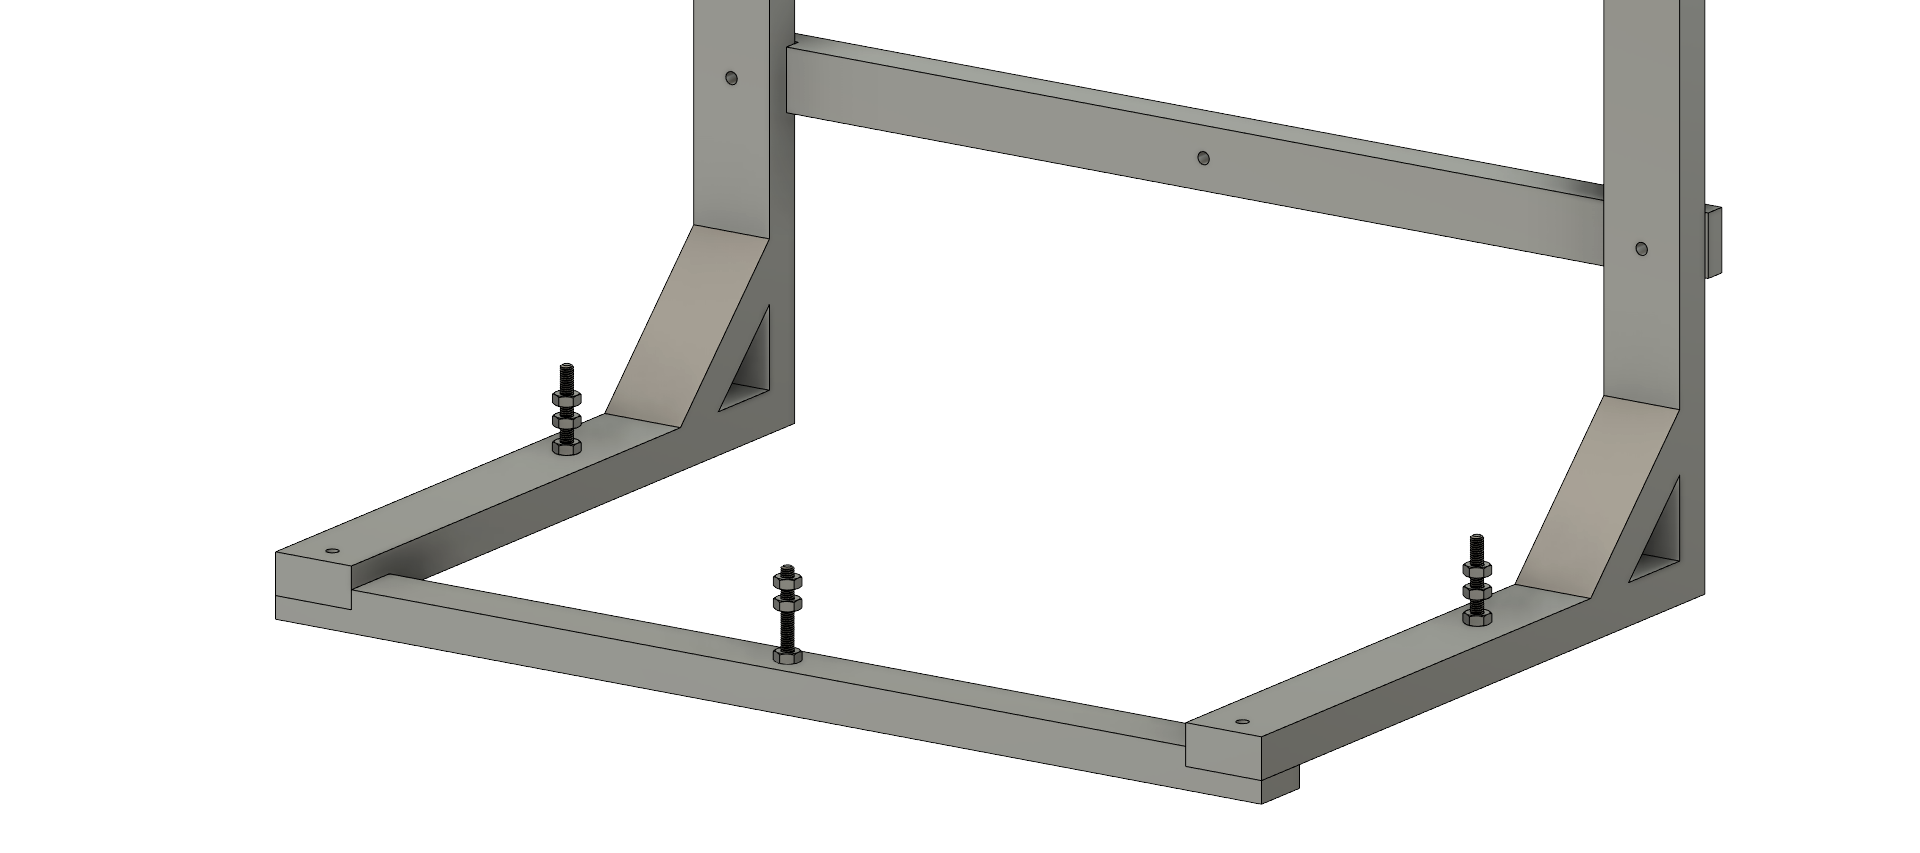
\includegraphics[width=12cm]{image/montage/boussole_solaire/6.png} 
\caption{cadran d'azimut}
\end{figure}

Le cadran d'azimut est imprimé sur du papier ordinaire puis plastifié pour résister aux intempéries, il est fixé sur la plaque de plexiglas grace à huit aimants qui permettent de faire coïncider les bords pour être parallèle avec la plaque de plexiglas et donc indirectement avec la barre transversale du cm121.\\

\begin{figure}[H]
\centering
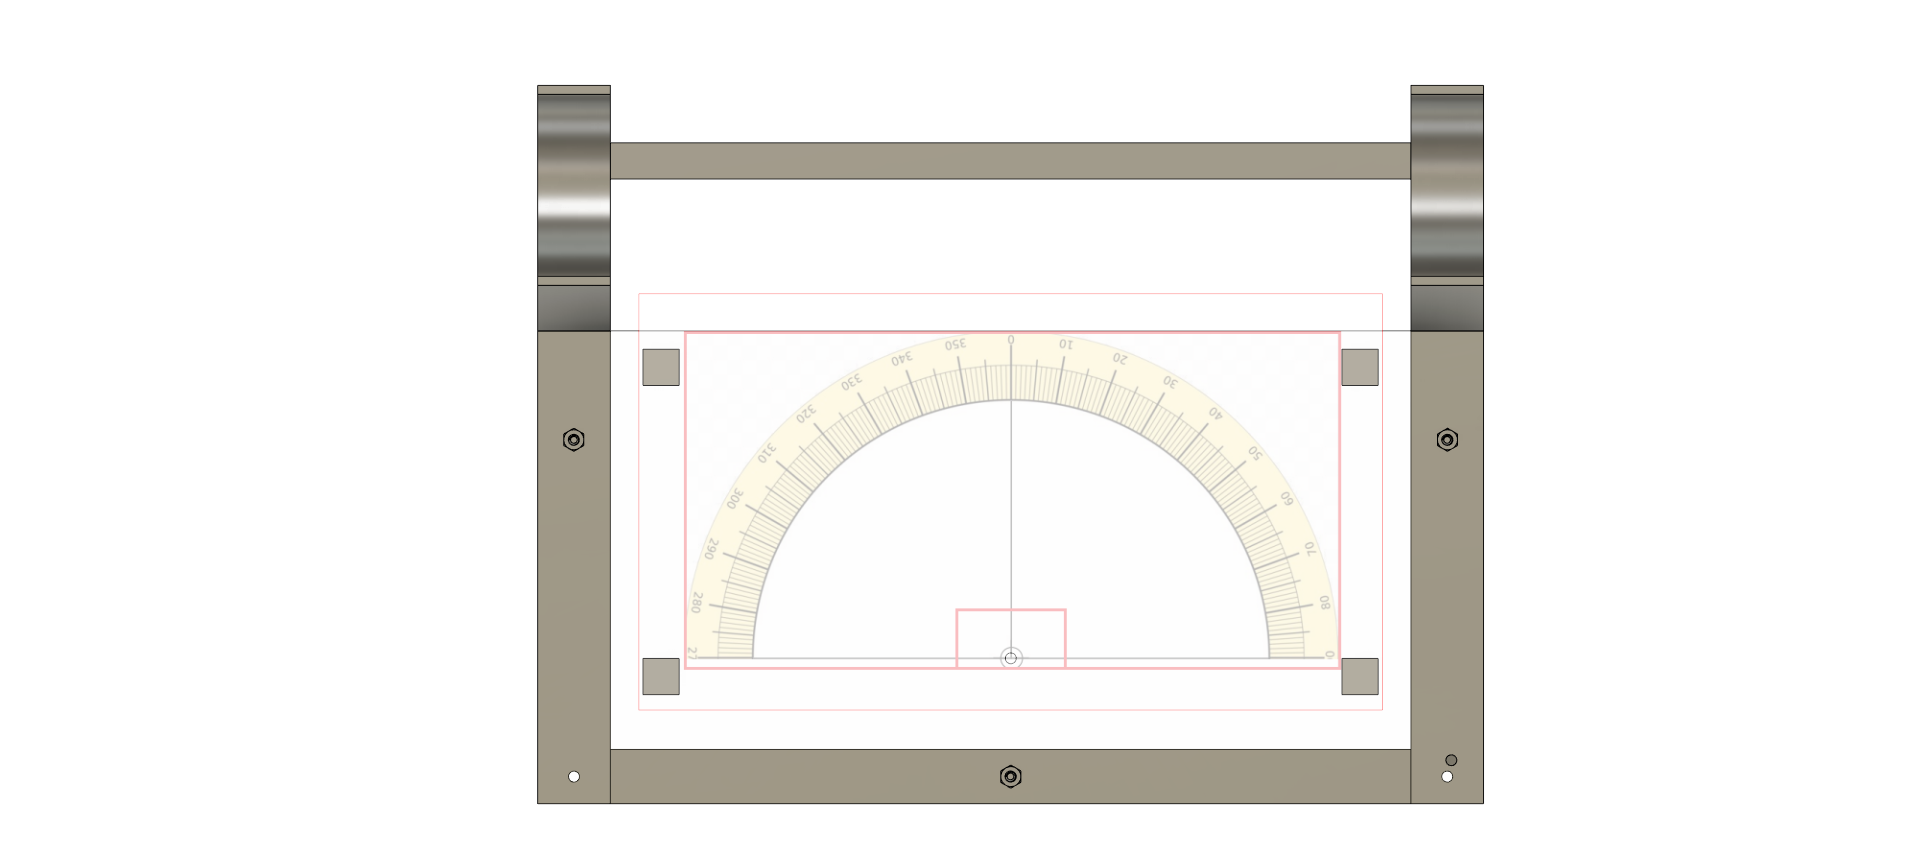
\includegraphics[width=12cm]{image/montage/boussole_solaire/5.png} 
\caption{cadran d'azimut}
\end{figure}


Viens ensuite la mise en place de la tige filetée de 3 mm qui supporte le fil. Le fil passe dans l'intersection du cadran d'azimut et la plaque de plexiglas par un trou de 3 mm, cela permet de réduire les effets du vent sur l'oscillation du fil.\\
Le cadran est par la suite fixé à la barre transversale à l'aide de Colliers rilsan, la plaque de plexiglas doit ensuite être réglée à l'horizontale, pour se faire un niveau de surface est utilisé et les ajustements se font par les trois boulons de 3*30mm.

 \begin{figure}[H]
\centering
\includegraphics[width=6cm]{image/montage/boussole_solaire/8.jpg} 
\caption{Boussole solaire installée sur le cm121}  
\end{figure}


Nous devons maintenant connaitre l'azimut du soleil, la solution la plus simple est d'utiliser un site internet comme par exemple suncalc.org. L'azimut obtenu doit ensuite être reporté sur le cadran, pour se faire il suffit de faire pivoter la base du cm121 sur son axe vertical. Le positionnement Nord-sud est effectué.\\
Cette méthode comporte quand même des limites, elle ne marche que pour les jours ensoleillés et la présence de masques cache à certains moments de la journée le soleil ce qui empêche le positionnement nord-sud. 
 

\subsection{Programmation}

J'ai dû développer lors du stage des programmes en python permettant de calculer le calendrier pour la maintenance du cm121, mais aussi d'effectuer l'analyse statistique d'une série de mesure.  Pour ce faire mes programmes permettant d'effectuer l'analyse statistique fonctionnent avec des dataframes, j'ai porté mon choix vers les dataframes car elles sont simples à manipuler.\\
~\\
Tous les programmes développés sont disponibles sur le github du LE2P [6].

\subsubsection{Calendrier du Cm121}

Le calendrier de maintenance du CM121 comporte deux informations, l'heure du midi solaire et la position de la barre coulissante.

La position de la barre coulissante est calculée en fonction de la déclinaison du soleil, par l'expression : 

\begin{flalign*}
&L = 297 tan (\delta)&&\\
\end{flalign*}
Avec :\\
L : la position de la barre coulissante\\
$\delta$ : la déclinaison du soleil\\
~~\\

Nous pouvons retrouver cette équation en calculant le côté opposé à l'angle aigu d'un triangle rectangle, comme sur la figure suivante:

\begin{figure}[H]
\centering
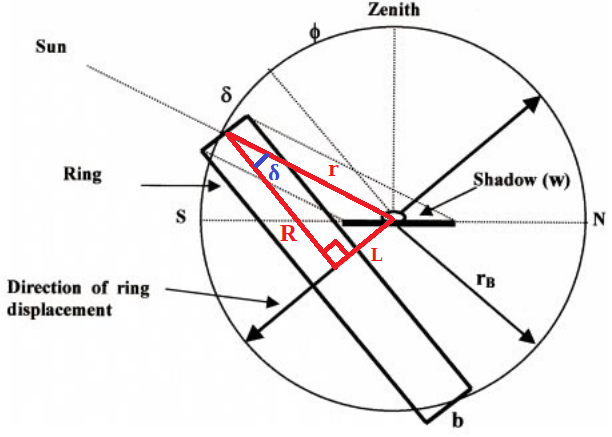
\includegraphics[width=8cm]{image/calendrier/1.PNG}  
\end{figure}

\begin{flalign*}
&R = 297~mm&&\\
&tan(\delta) = \frac{L}{R}&&\\
&L = R~tan(\delta)&&\\
&L = 297tan(\delta)&&\\
\end{flalign*}

Le programme calcul aussi les maintenances minimums à éffectuer en se basant sur la déclinaison du soleil. Etant donner que la position de la barre coulissante est obtenue en fonction de la déclinaison nous pouvons calculer les jours de maintenance minimun au cours de l'année. Pour se faire on place la barre coulissante pour le jour correspondant (la position normale), puis nous deplacons la barre pour obtenir l'ombre à 0.5mm du dome en verre du pyranometre (la position limite).

\begin{figure}[H]
    \begin{minipage}[c]{.46\linewidth}
        \centering
        \includegraphics[width=8cm]{image/calendrier/6.jpg} 
        \caption{Position normale}
    \end{minipage}
    \hfill%
    \begin{minipage}[c]{.46\linewidth}
        \centering
        \includegraphics[width=8cm]{image/calendrier/5.jpg} 
        \caption{Position limite}
    \end{minipage}
\end{figure}


Il suffit maintenant de savoir la déclinaison pour la position normale et la position limite, pour savoir la déclinaison de la position limite il nous suffit de lire la position de la barre coulissante et de regarder sur notre calendrier de maintenance à quel jour elle correspond et de calculer la déclinaison. On peut désormais calculer la différence des déclinaisons.\\

\begin{flalign*}
&\Delta \delta=\delta_{position~normale}-\delta_{position~limite}&&\\
&\Delta \delta=1.3^\circ&&\\
\end{flalign*}

Nous trouvons un delta de 1.3°, cela signifie que si la déclinaison subit une variation de $\pm 1.3^\circ$ entre la derniere maintenance et aujourd'hui nous devons repositionner la barre coulissante.\\
~\\
Le programme retourne alors trois calendriers, un calendrier au format csv, un calendrier au format xlsx et un calendrier ics. Le calendrier csv est obtenu par du texte brut ce qui signifie qu'il fonctionne avec tous les logiciels de traitement de texte, mais ce format ne permet pas la mise en forme. Le calendrier xlsx permet d'intégrer la mise en forme au calendrier, nous obtenons ainsi des codes couleurs, en vert les jours fériés, en bleu les weekends et en rouge les maintenances minimums à effectuer sur le cm121. Le calendrier ics permet d'avoir les positions du cm121 au format iCalendar ce qui permet entre autres d'avoir le midi-solaire, la position de la barre coulissante et les maintenance minimum via son smartphone.\\

\begin{figure}[H]
\centering
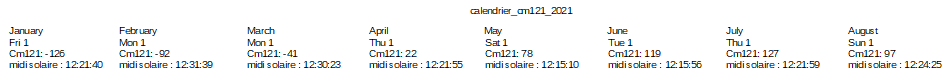
\includegraphics[width=16cm]{image/calendrier/3.PNG} 
\caption{calendrier au format csv}  
\end{figure}

\begin{figure}[H]
\centering
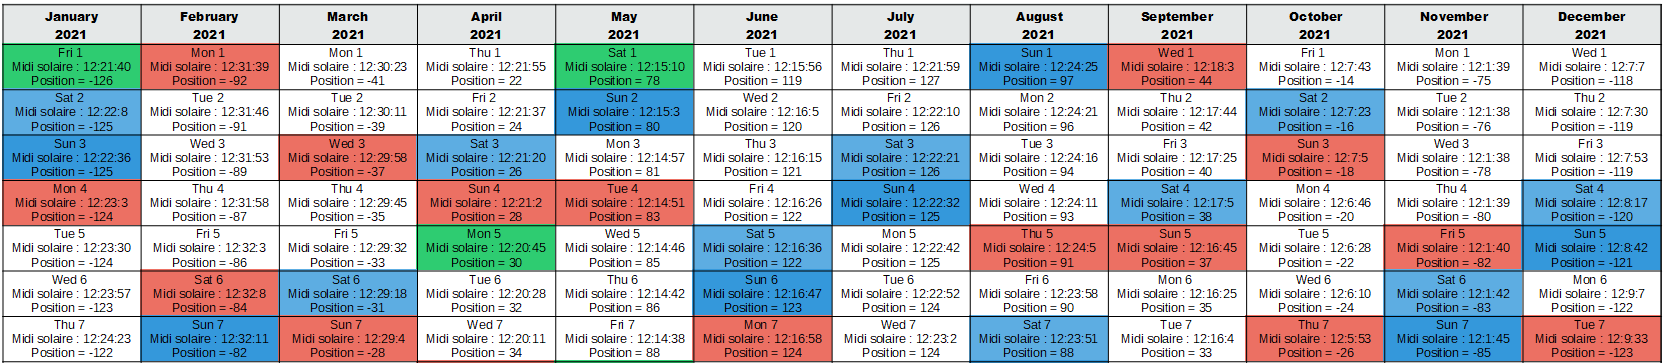
\includegraphics[width=16cm]{image/calendrier/2.PNG} 
\caption{calendrier au format xlsx}  
\end{figure}


\begin{figure}[H]
    \begin{minipage}[c]{.46\linewidth}
        \centering
        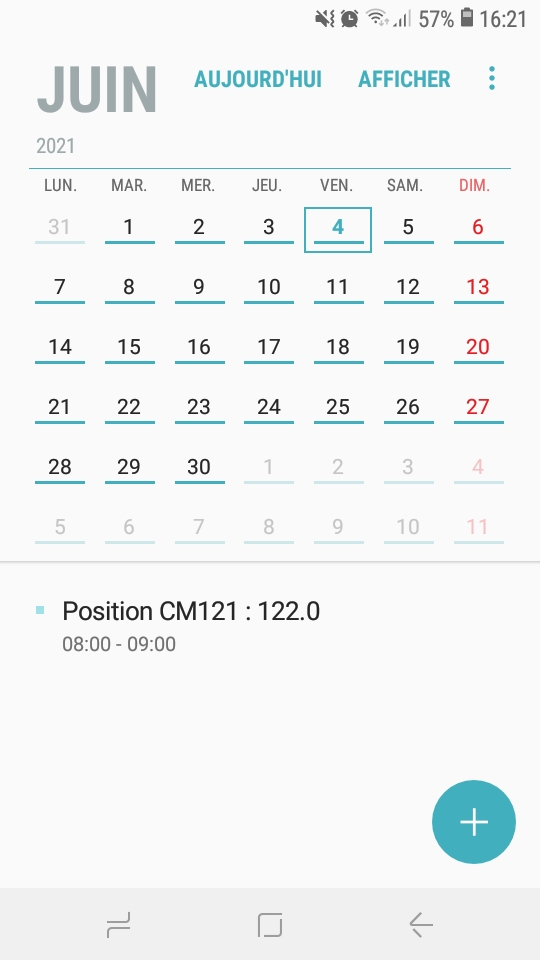
\includegraphics[width=5cm]{image/calendrier/4.jpg} 
		\caption{calendrier au format ics}
    \end{minipage}
    \hfill%
    \begin{minipage}[c]{.46\linewidth}
        \centering
        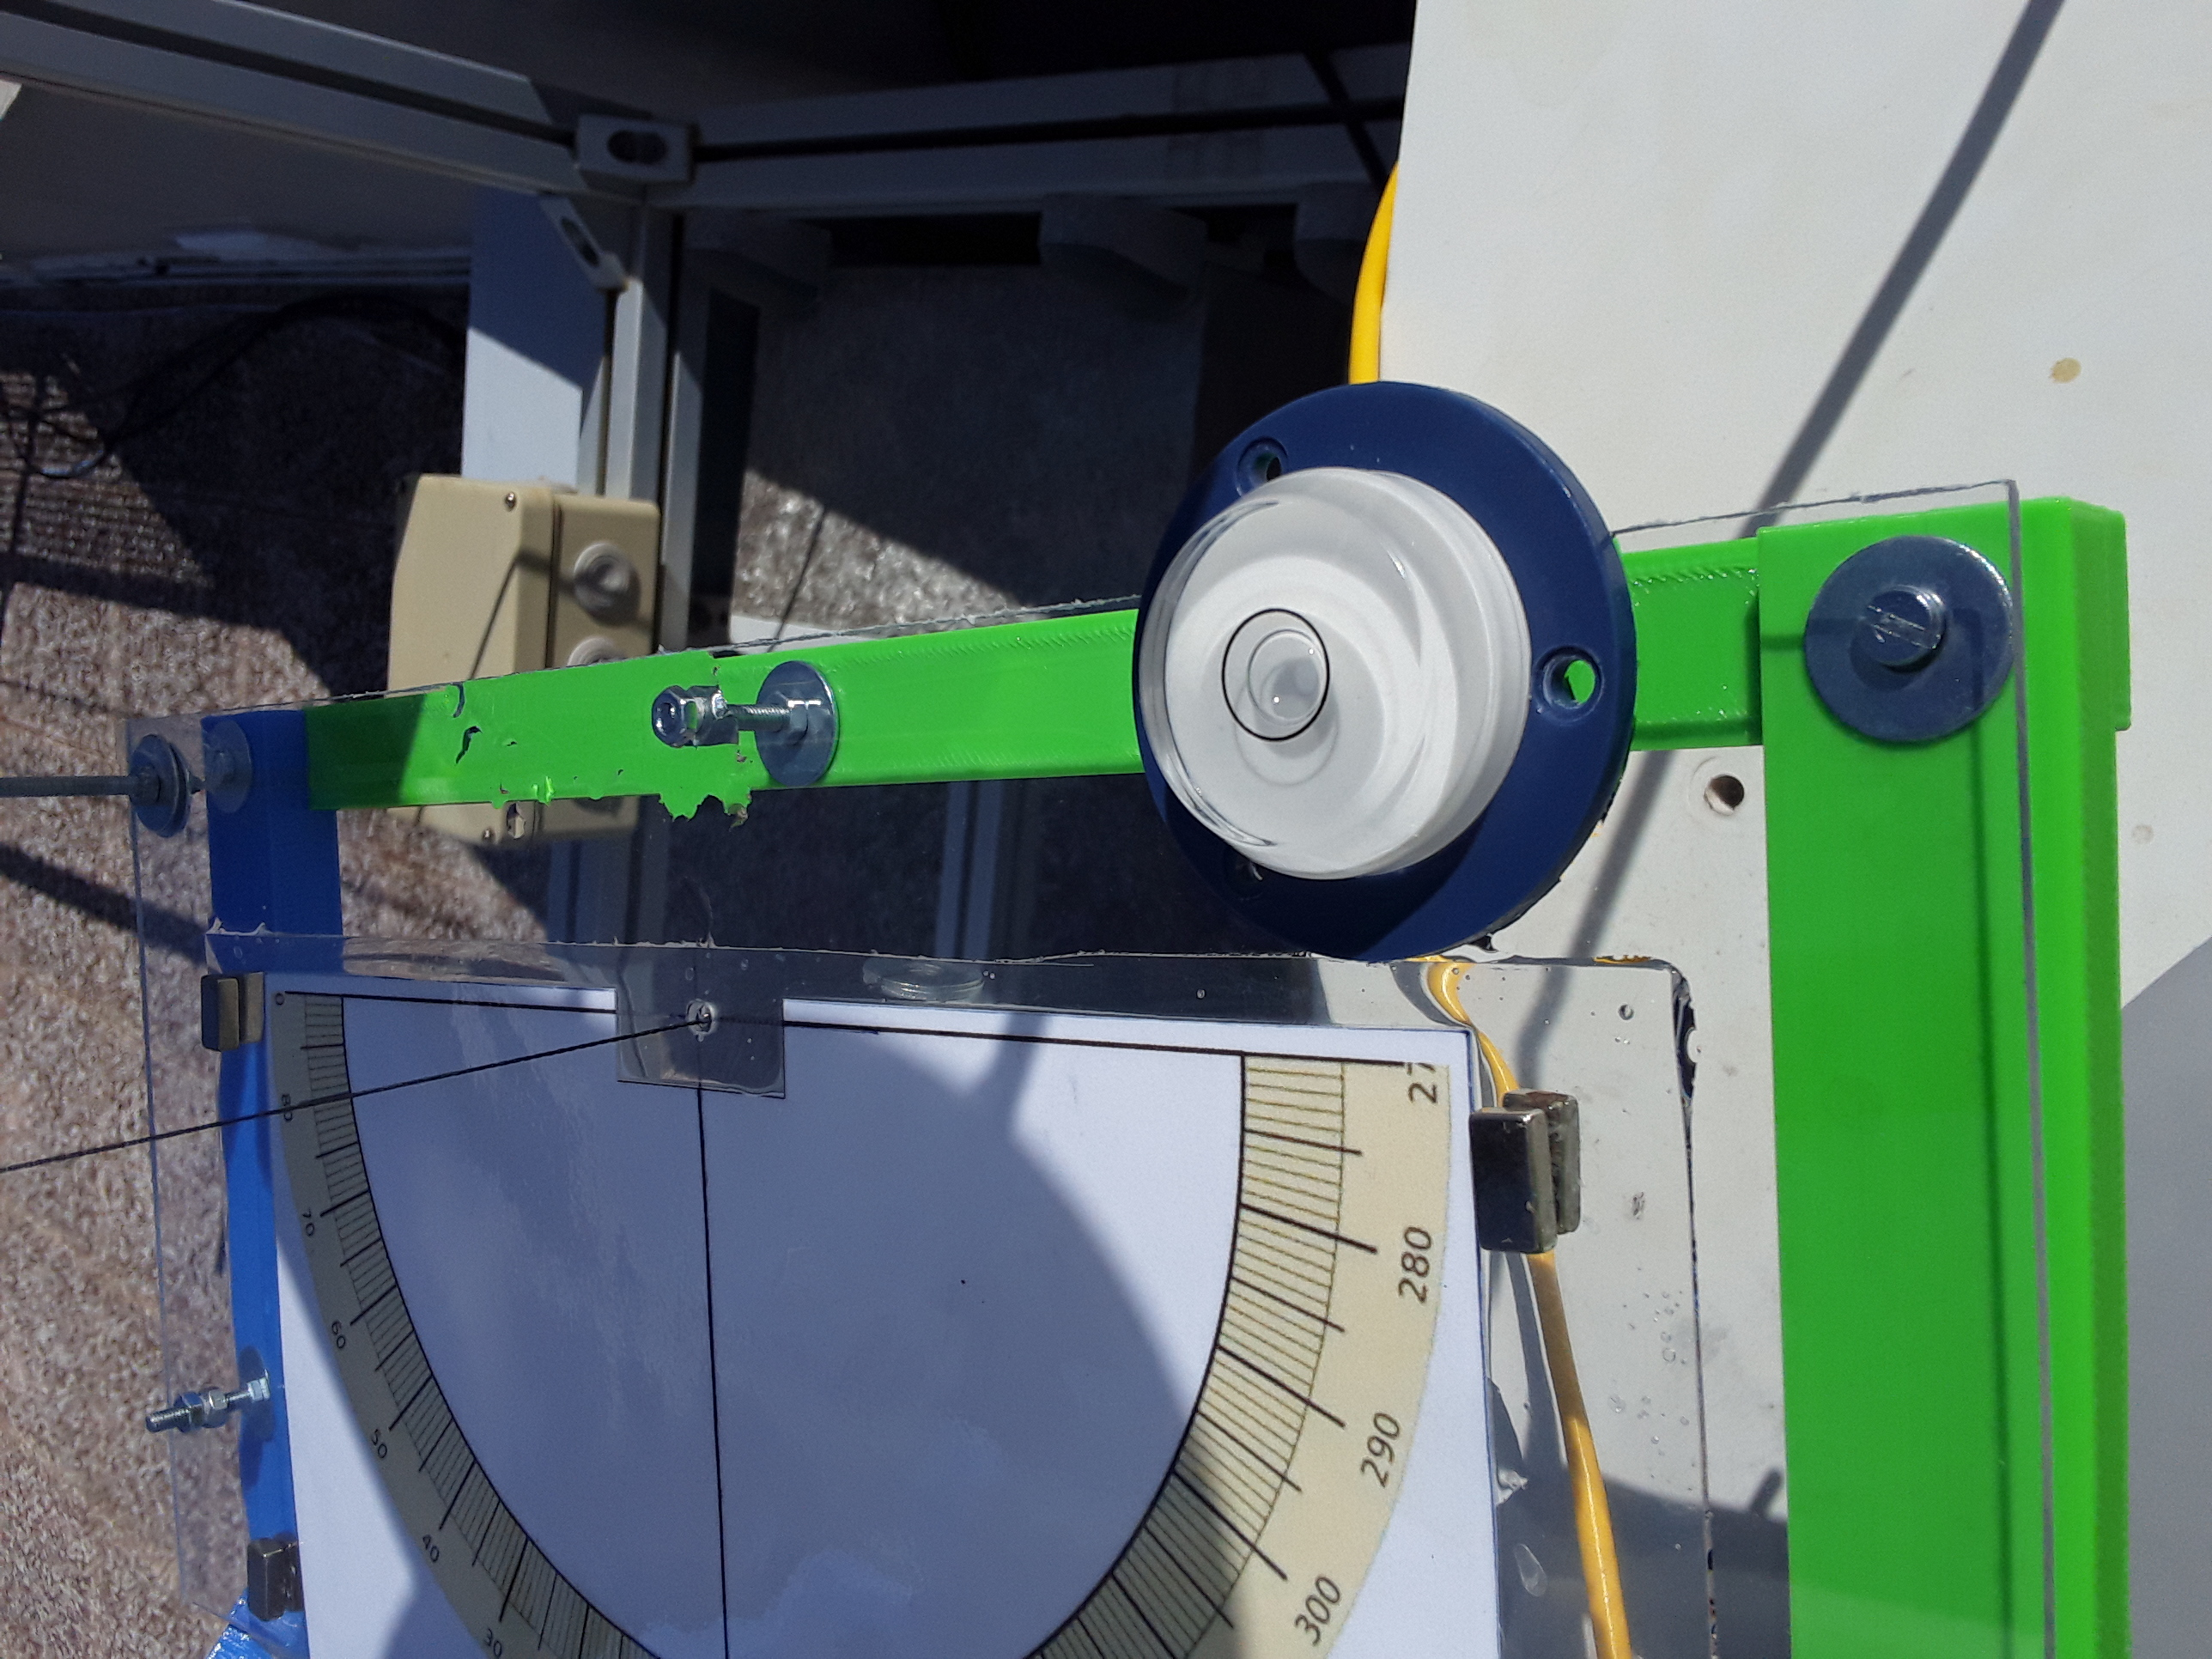
\includegraphics[width=5cm]{image/calendrier/7.jpg} 
        \caption{calendrier au format ics, maintenance minimum}
    \end{minipage}
\end{figure}

\subsubsection{Suppression des données non utilisés, non acquis et abérantes}

Le fichier de mesure comporte généralement des données non acquises pouvant bloquer l'exécution de certains programmes, mais aussi les données pour la nuit qui sont inintéressantes dans le cas du DHI ou du GHI, la création d'une fonction pour supprimer ces mesures fut nécessaire.

\subsubsection{Calcul des facteurs de correction}

Les données du cm121 doivent être corrigées car l'arc d'ombrage masque une partie du diffus. L'expression permettant de calculer le facteur de correction donné dans la datasheet se base sur les travaux de Drummond (1956). Cette correction fait l'hypothèse que le ciel est isotropique ce qui donne une correction des mesures purement géométrique (voire annexe).\\

Les mesures du CM121 sont corrigées par une fonction qui calcule le facteur de correction en se basant sur l'heure ou la mesure a été prise et l'applique par la suite aux mesures.

\subsubsection{Analyse statistique et étalonnage}

Lors de l'étalonnage les mesures subissent une régression linéaire par rapport à des mesures de références, nous obtenons alors une droite d'équation $y = ax + b$ que nous voulons ramener pour obtenir une droite d'équation $y = x$.\\
~\\
La fonction développé permet d'effectuer l'étalonnage mais aussi l'analyse statistique. L'analyse statistique permet d'obtenir sur le graphique le coefficient de détermination $R^2$, la variance, l'erreur quadratique moyenne et l'erreur absolue moyenne.\\
~\\
Le coefficient de détermination $R^2$ est un indicateur qui permet de juger la qualité d’une régression linéaire. Si le $R^2$ vaut 1, cela signifie que l’équation de la droite de régression est capable de déterminer 100 \% de la distribution des points. Cela signifie alors que le modèle mathématique utilisé, ainsi que les paramètres "a" et "b" calculés sont ceux qui déterminent la distribution des points.\\
~~\\
La variance permet de mesurer la dispersion des valeurs d'un échantillon, plus elle est élevée, plus la dispertion est élevée. On définit la variance d'une variable discrète composée de n observations comme suit :\\

\begin{flalign*}
&\sigma ^2 =  \frac{\sum(X+\overline{X})^2}{n}&&\\
& \overline{X} : moyenne&&\\
& X : valeur incluse dans l'ensemble de données&&\\
\end{flalign*}

~~\\
L'erreur quadratique moyenne (RMSE) fournit une indication par rapport à la dispersion ou la variabilité de la qualité de la prédiction, il est souvent relié à la variance car les valeurs de RMSE sont difficiles à interpréter parce que l’on n'est pas en mesure de dire si on a une variance faible ou forte, l'erreur quadratique moyenne donne plus de poids aux erreurs élevés. On définit l'erreur quadratique moyenne comme suit :

\begin{flalign*}
&RMSE = \sqrt{\frac{1}{N}  \overset{N}{\underset{i=1}{\sum}} (\widehat{y}_i -y_i)^2 }&&
\end{flalign*}
~\\ 

L'erreur absolue moyenne (MAE) représente l'erreur systématique, toutes les différences individuelles ont le même poids.\\

\begin{flalign*}
&MAE = \frac{1}{N}  \overset{N}{\underset{i=1}{\sum}} |\widehat{y}_i -y_i| &&
\end{flalign*}


~\\
La fonction renvoie le graphique ci-dessous.

\begin{figure}[H]
\centering
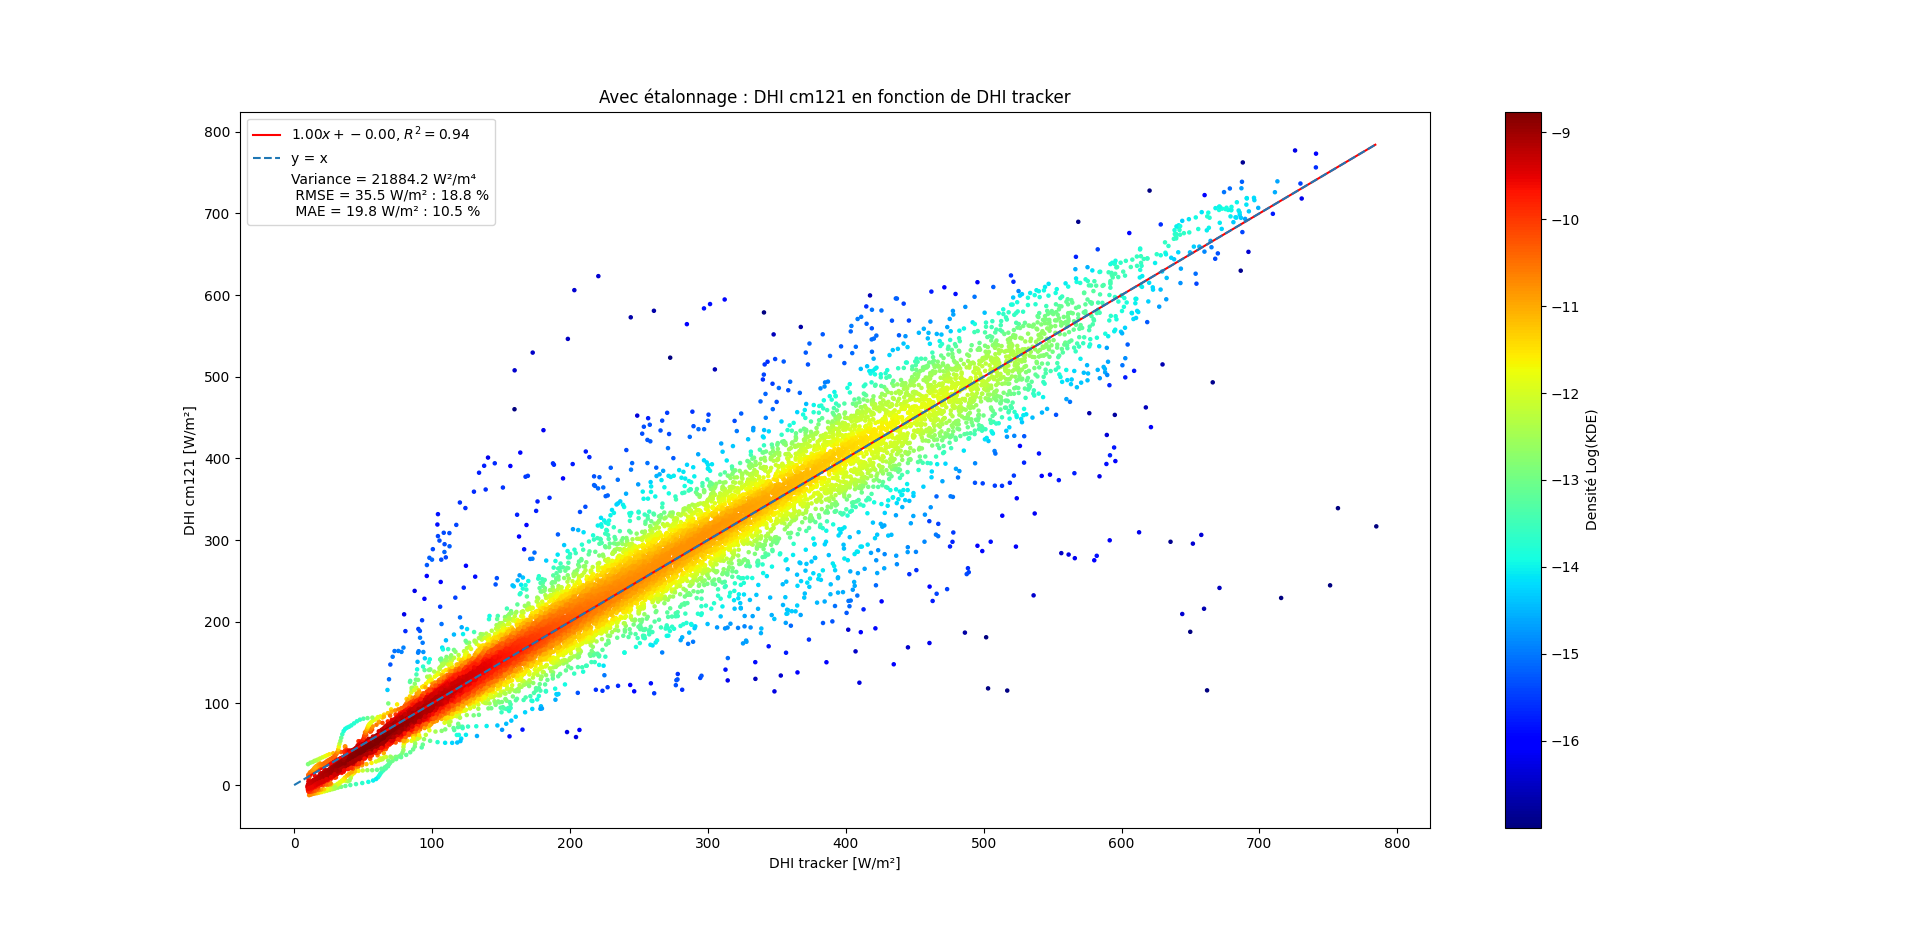
\includegraphics[width=15cm]{image/etallonnage/1.png} 
\caption{régression linéaire pour mars 2021}  
\end{figure}

\subsubsection{Représentation graphique de l'erreur relative}

Il est intéressant d'avoir la représentation de l'erreur relative en fonction de l'azimut et de l'élévation du soleil, cela permet de mettre en lumière des journées particulières comme par exemple le dysfonctionnement de l'acquisition des mesures, mais aussi la présence de masques ou de reflet impactant le pyranomètre. Les erreurs aberrantes qui sont identifées grace à cette méthode peuvent donc être supprimées.\\
La fonction renvoie le graphique ci-dessous.
 
\begin{figure}[H]
\centering
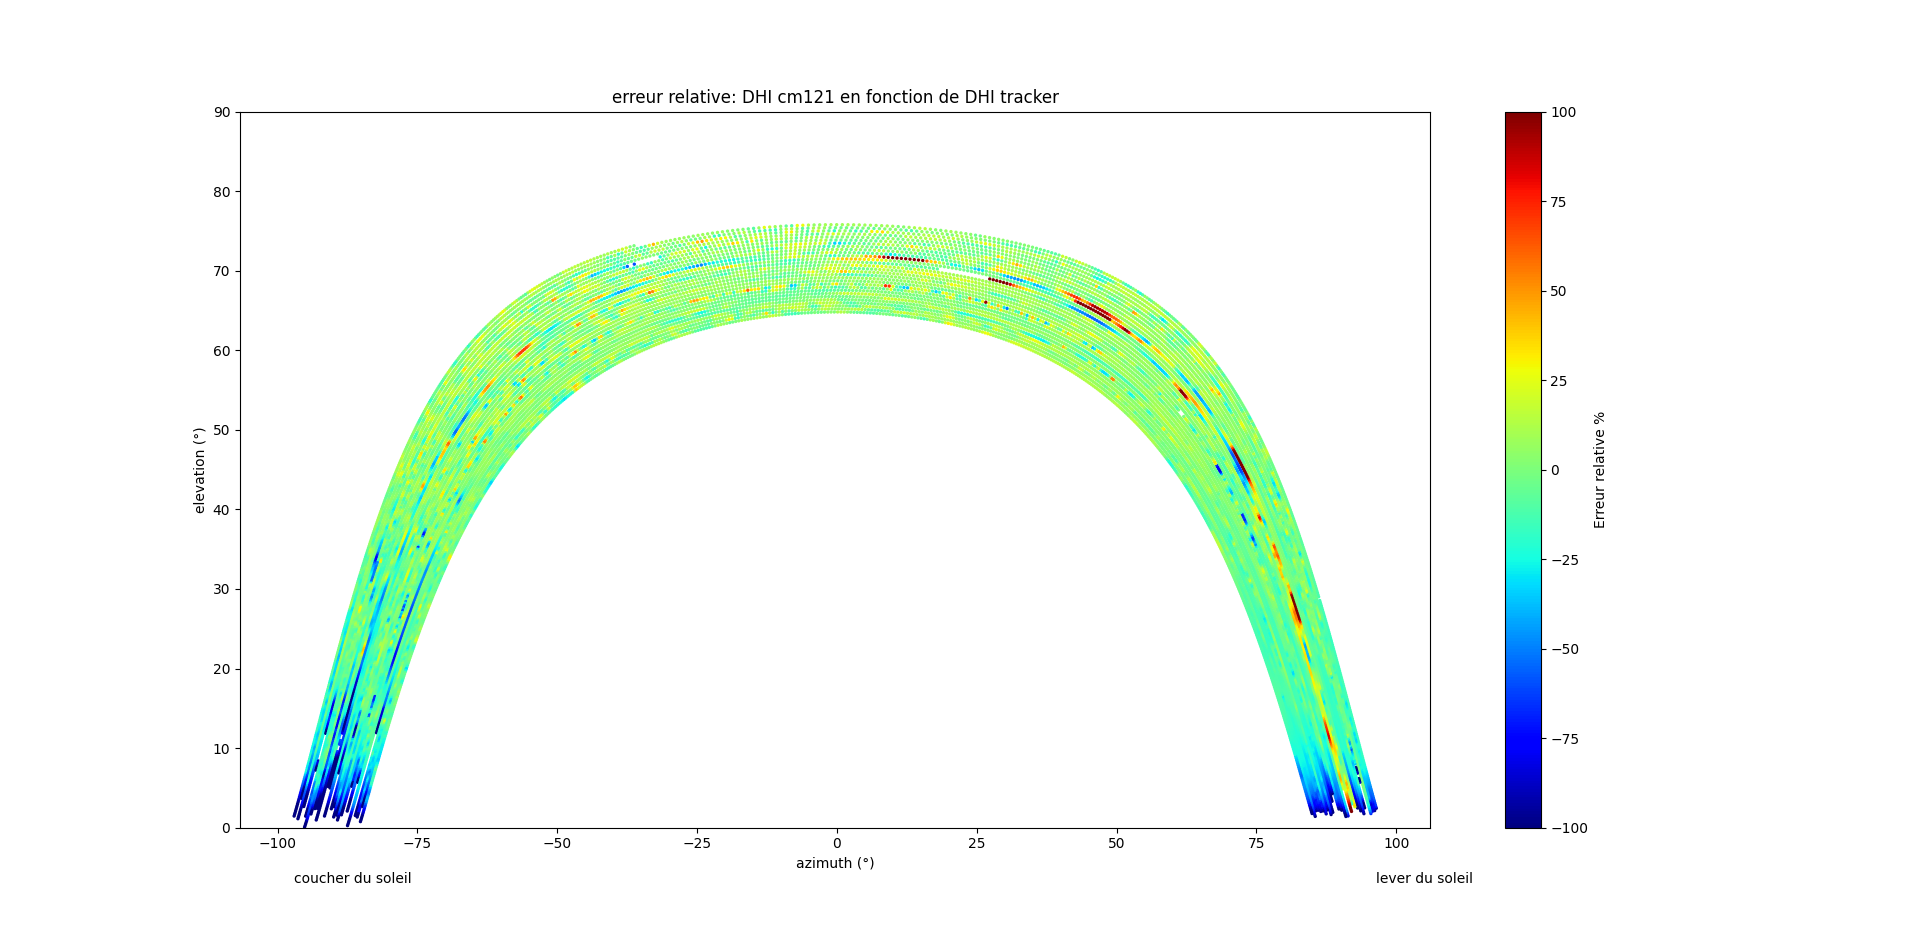
\includegraphics[width=15cm]{image/erreur_relative/1.png} 
\caption{erreur relative}  
\end{figure}

\subsubsection{Histogramme}

La dernière fonction pour l'analyse statistique donne la représentation graphique de la répartition d'une variable, dans notre cas la fonction donne la répartition du rayonnement diffus et de l'erreur relative.\\
Elle renvoie les graphiques ci-dessous.
\begin{figure}[H]
\centering
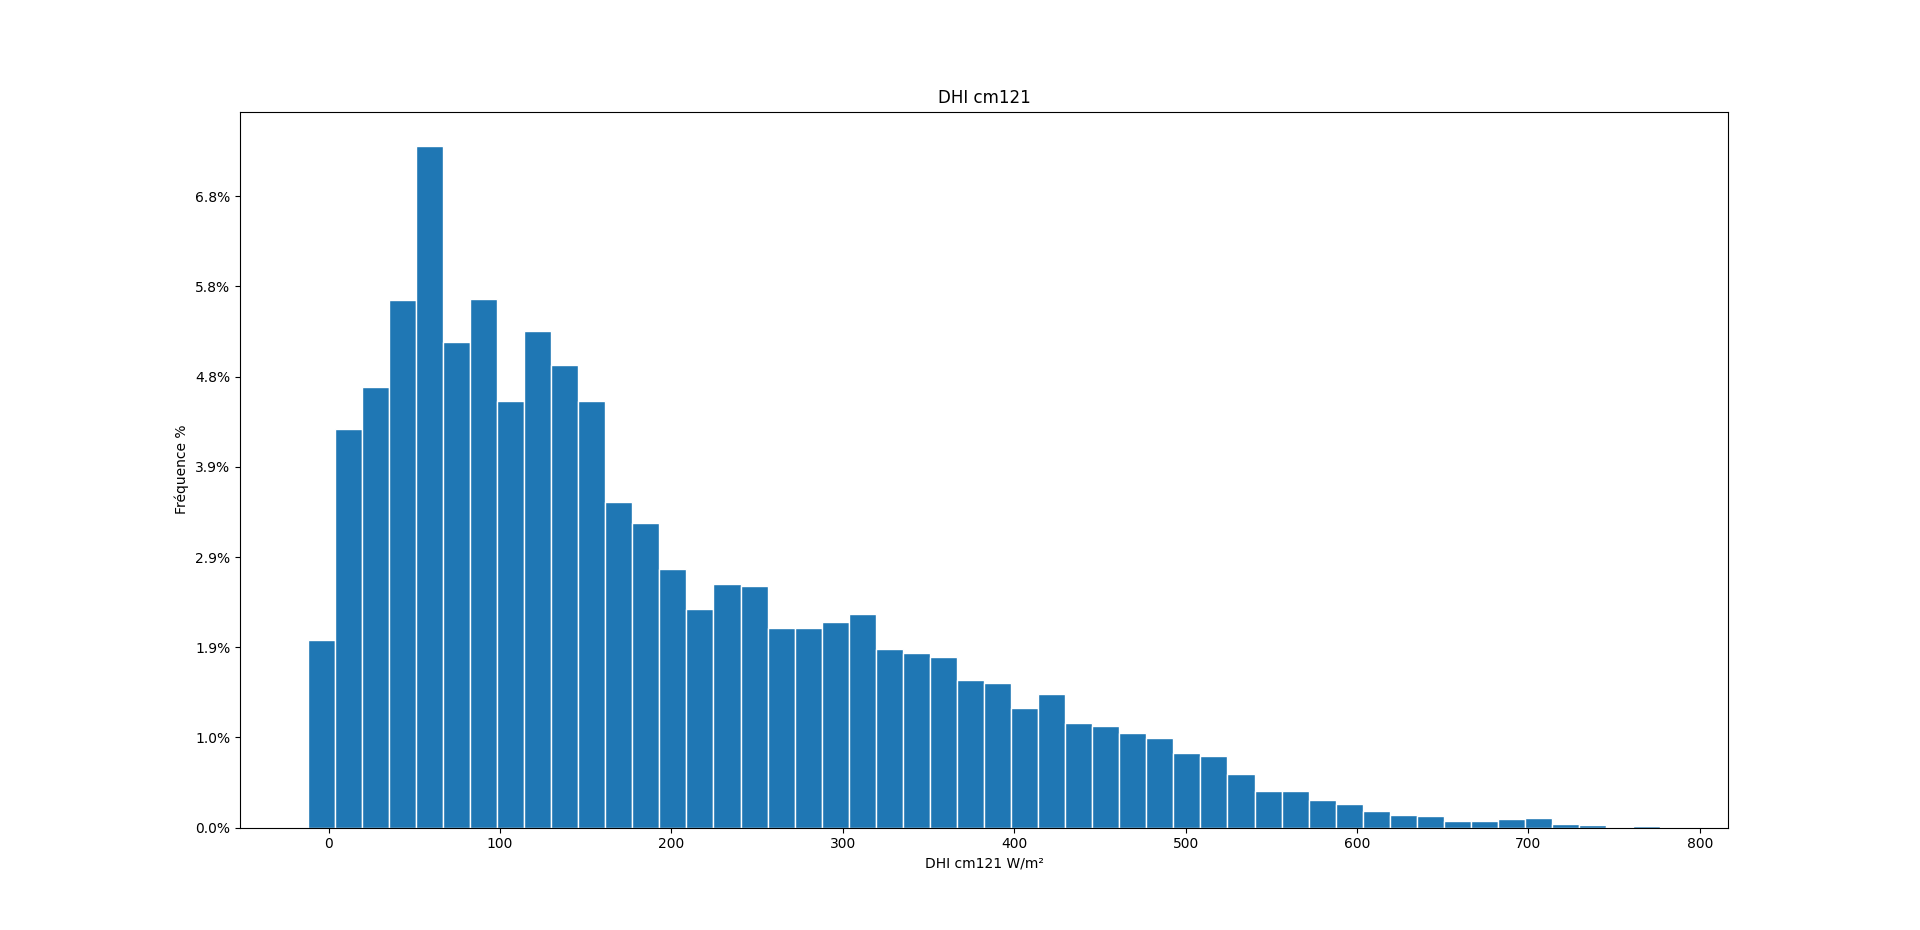
\includegraphics[width=15cm]{image/histogramme/1.png} 
\caption{régression linéaire}  
\end{figure}

\begin{figure}[H]
\centering
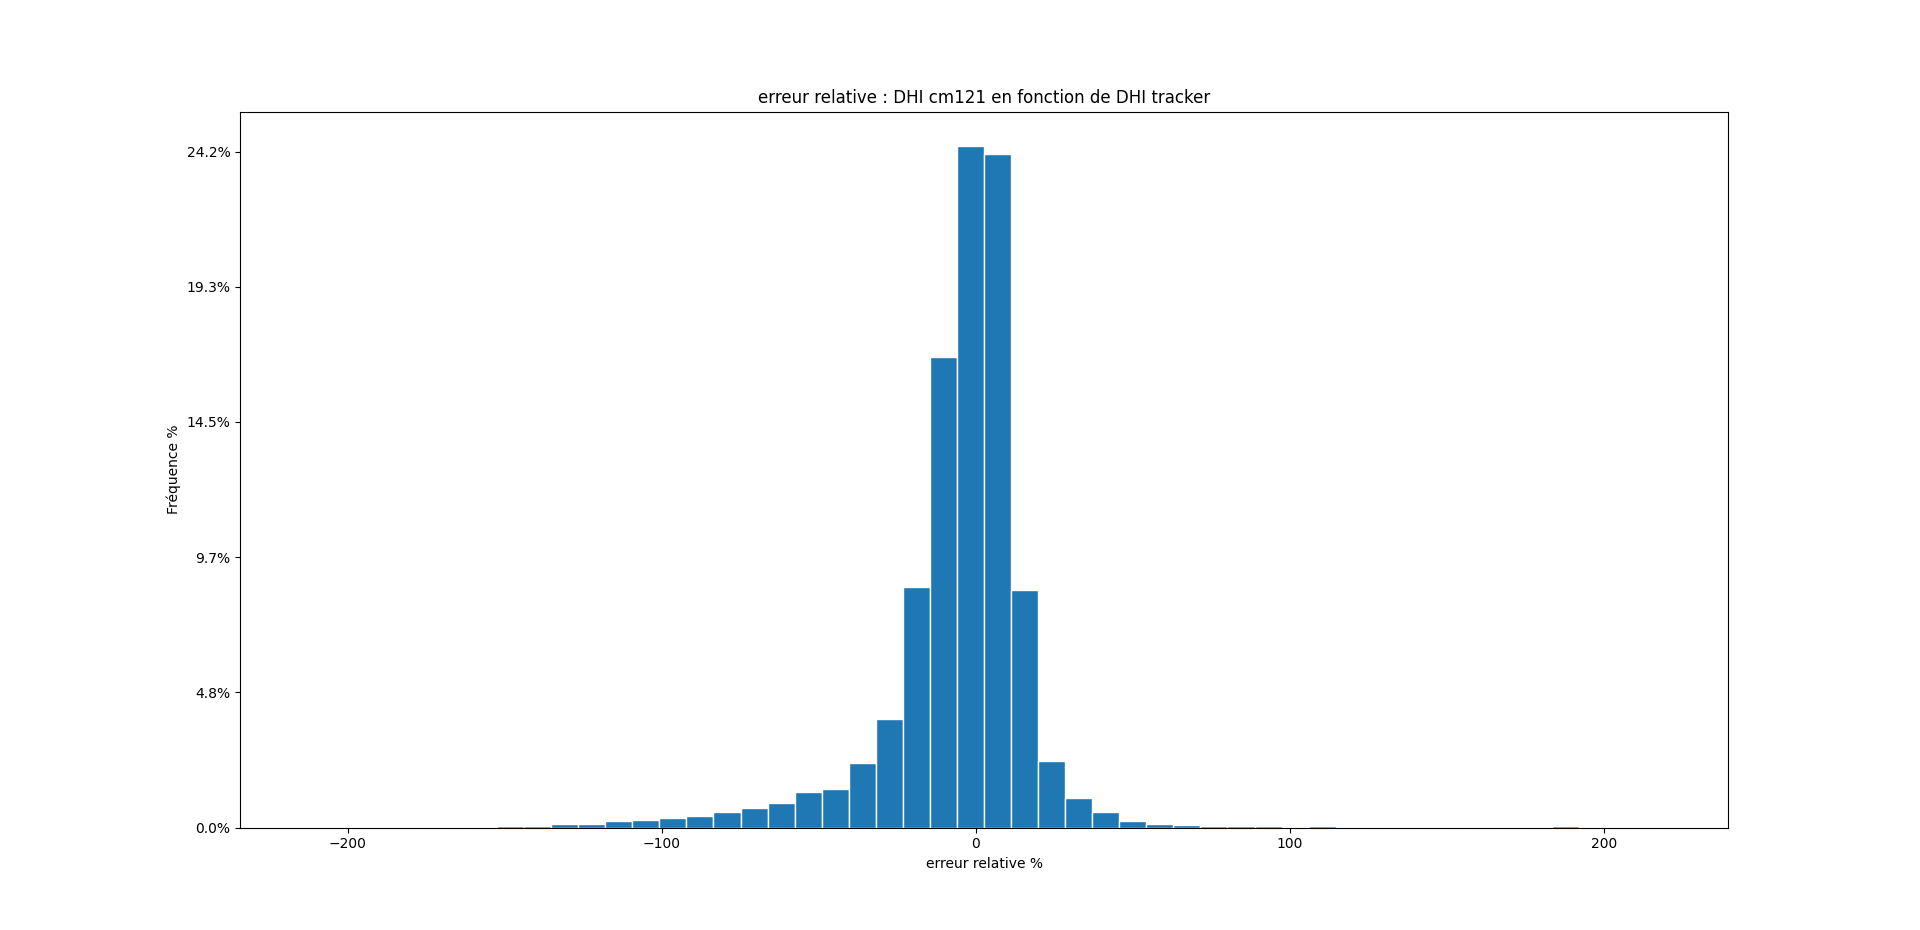
\includegraphics[width=15cm]{image/histogramme/2.png}  
\caption{régression linéaire}  
\end{figure}

\subsubsection{Selection des mesures entre deux intervalles}

Deux fonctions ont été créer pour sélectionner les mesures entre une période donnée, la première permet d'avoir les mesures entre deux dates et la dernière permet d'avoir les mesures pour une tranche horaire spécifiée.

\subsubsection{éxécution de l'analyse statistique}

Pour faciliter l'utilisation du programme celui-ci s'exécute via un terminal, pour ce faire l'utilisateur doit juste renseigner le nom de son fichier de mesure, choisir les valeurs pour la mesure et les valeurs pour la référence. Si l'utilisateur le souhaite il est aussi en mesure de renseigner la période sur laquelle il souhaite l'analyse statistique.


\subsubsection{Etallonage du cm121 avec le spn1}

Pour effectuer l'étalonnage du cm121, les mesures de référence sont celles du tracker. Nous cherchons à savoir si les mesures du CM121 sont plus proches du spn1 ou du tracker, si les mesures sont plus proche de celle du spn1 alors il semble préférable d'effectuer l'étalonnage avec les mesures du spn1. Le CM121 et le spn1 utilise tous deux un arc pour masquer le rayonnement direct du soleil, cet arc donne un angle de vue de 10.8° pour le cm121 et le spn1, alors que le masque du tracker donne un angle de vue de 5°.\\
L'analyse statistique est éffectuée entre le 01 janvier 2021 jusqu'au 01 avril 2021.

\begin{figure}[H]
\centering
\includegraphics[width=15cm]{image/comparaison_cm121_spn1/cm121_tracker_2021-01-01_2021-04-01/regression_avec_étalonnage_DHI cm121vsDHI tracker.png} 
\caption{cm121 en fonction du tracker}  
\end{figure}

\begin{figure}[H]
\centering
\includegraphics[width=15cm]{image/comparaison_cm121_spn1/cm121_spn1_2021-01-01_2021-04-01/regression_avec_étalonnage_DHI cm121vsDHI spn1.png}  
\caption{cm121 en fonction du spn1}  
\end{figure}

On constate que les variances sont approximativement les mêmes, qui plus est en étalonnant le cm121 avec le spn1 l'erreur quadratique moyenne et l'erreur absolue moyenne sont plus faibles et le coefficient de détermination est plus élevé. Les mesures du cm121 sont donc plus proches des mesures du spn1 que celles du tracker, il est donc possible d'étalonner le cm121 avec le spn1.  

\subsubsection{Impact de la ventillation sur les mesures du cm121}

Les mesures avec la ventilation opérationnelle ont été acquise entre le 21 avril 2021 et le 31 mai 2021, nous devons donc comparer les mesures avec ventilation et sans ventilation sur une même période de 41 jours, les mesures entre le 21 avril 2021 et le 31 mai 2021 (avec ventillation) sont comparées aux mesures entre le 11 mars et le 20 avril (sans ventillation).

\begin{figure}[H]
\centering
\includegraphics[width=15cm]{image/impact_ventillation/avril_mai_2021/regression_avec_étalonnage_DHI cm121vsDHI tracker.png} 
\caption{régression linéaire période avec ventillation}  
\end{figure}

\begin{figure}[H]
\centering
\includegraphics[width=15cm]{image/impact_ventillation/archive_2021-03-11_2021-04-20/regression_avec_étalonnage_DHI cm121vsDHI tracker.png}  
\caption{régression linéaire période sans ventillation}  
\end{figure}

\begin{figure}[H]
\centering
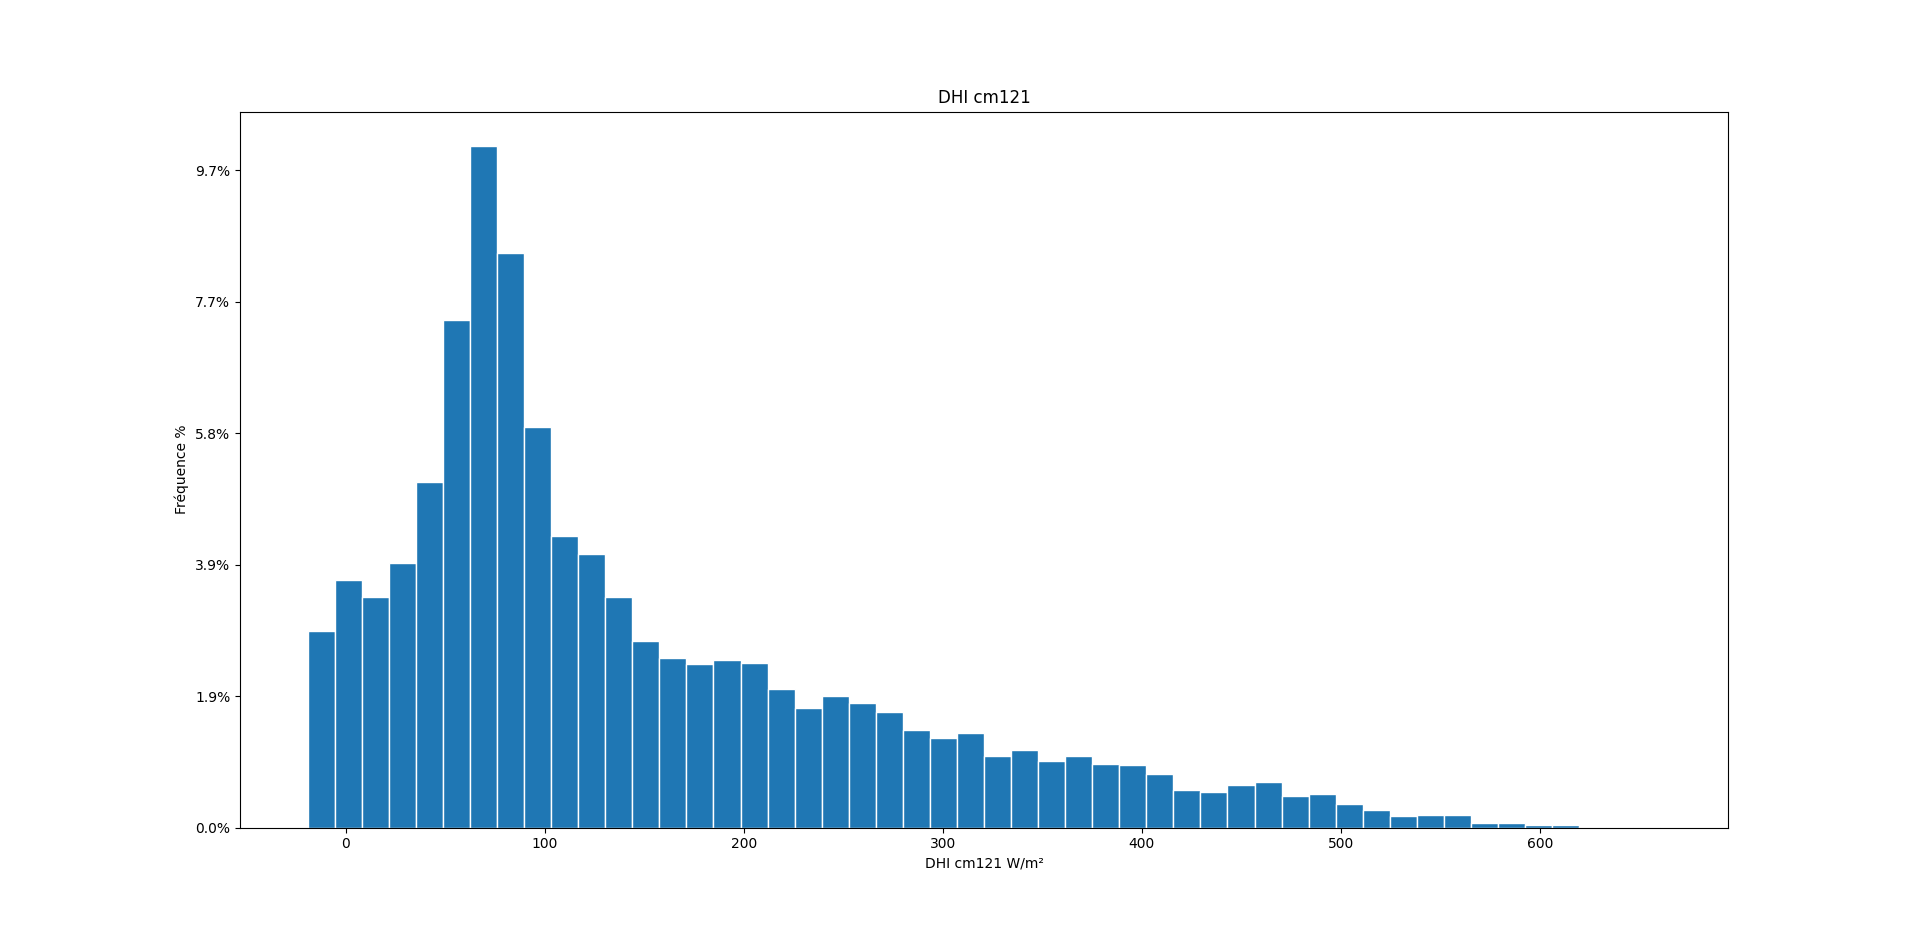
\includegraphics[width=15cm]{image/impact_ventillation/avril_mai_2021/histogramme_3.png}  
\caption{répartition du DHI avec ventillation}  
\end{figure}

\begin{figure}[H]
\centering
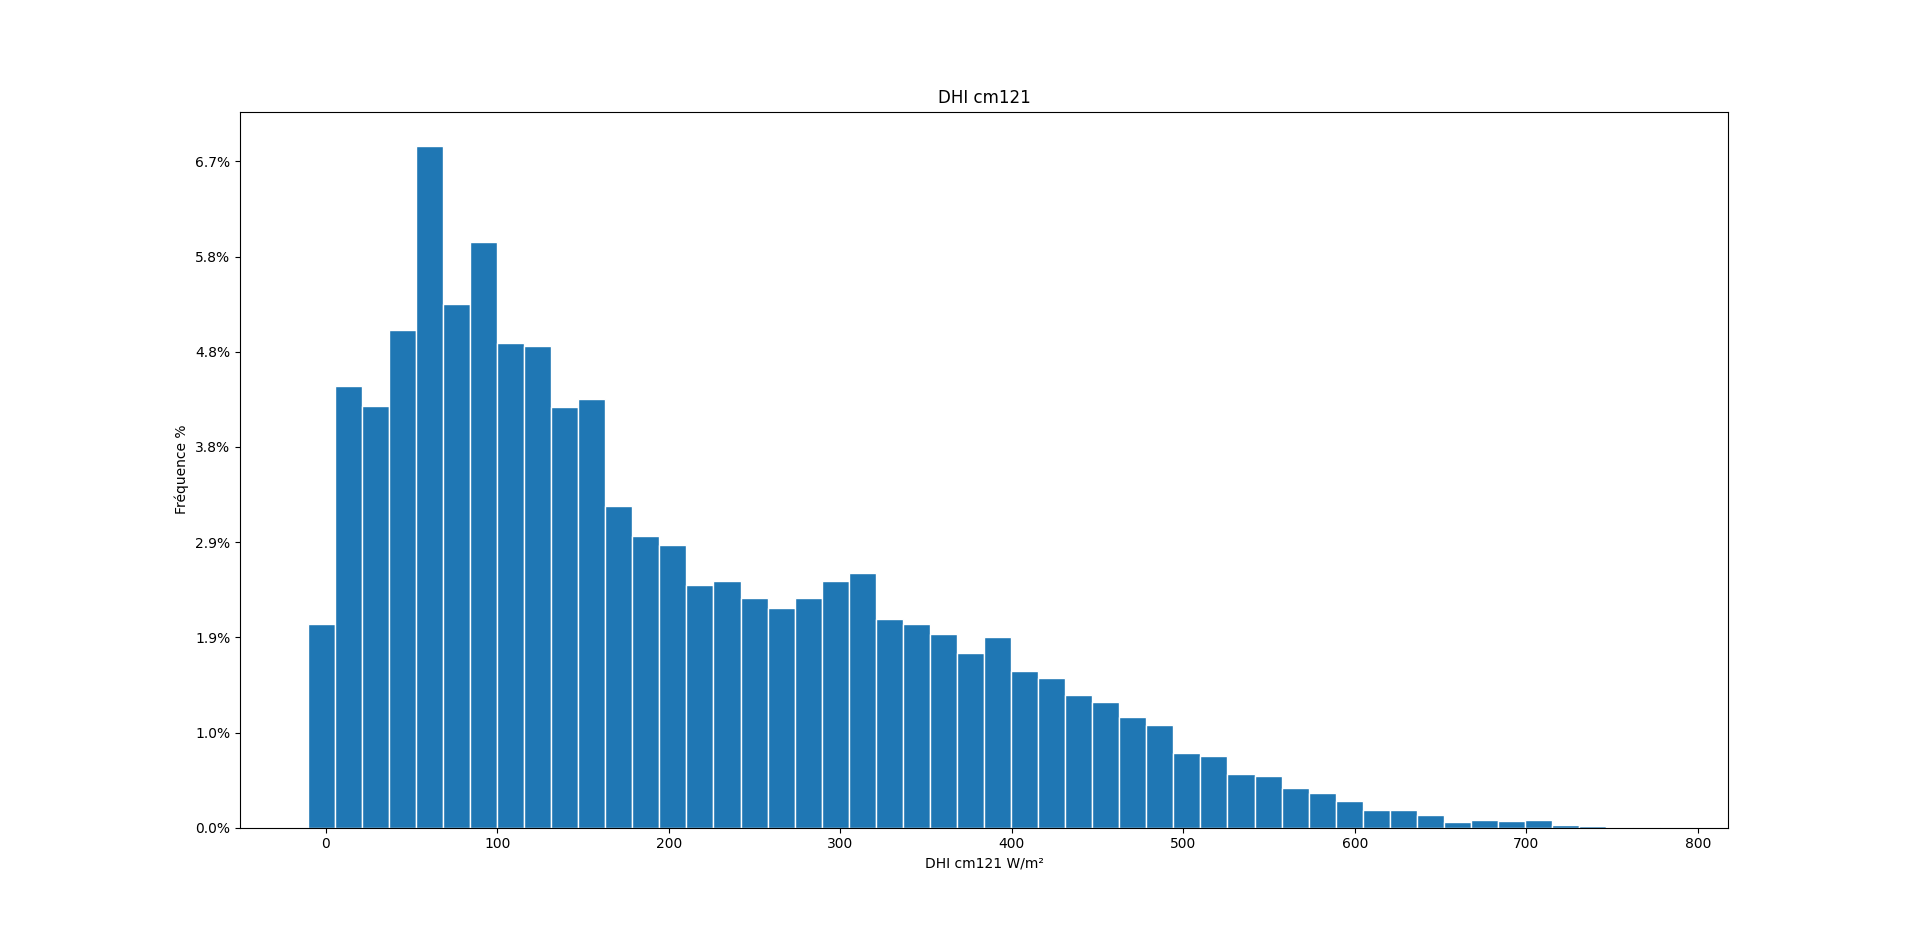
\includegraphics[width=15cm]{image/impact_ventillation/archive_2021-03-11_2021-04-20/histogramme_3.png} 
\caption{répartition du DHI sans ventillation}  
\end{figure}

Les histogrammes nous montrent que pour les deux périodes la répartition du DHI est similaire.
Nous obtenons avec la mise en place de la ventilation un RMSE et un MAE plus élevé, en revanche la variance est plus faible, les mesures ont donc moins de dispersion avec la ventilation. Pour obtenir des résultats plus concrets il faudrait réaliser la même étude sur une période plus longue.

\subsection{Les apports du stage}

Le stage m'a permis de découvrir un nouveau langage de programmation, ainsi que l'utilisation de github qui permet d'enregistrer les différentes versions de son projet, mais aussi les bonnes pratiques que ce soit pour la programmation ou l'organisation de son répertoire de travail. J'ai également pu apprendre l'utilisation d'un logiciel de modélisation 3D ainsi que le principe de la boussole solaire.


\section{Conclusion}

Le stage a mis en lumière que les mesures du cm121 sont plus proches du spn1 que du tracker, l'étude statistique a montré une variance similaire dans le cas ou le cm121 est comparé au tracker et dans le cas ou le cm121 est comparé au spn1, ce qui signifie que dans les deux cas la dispersion des mesures est la même. La comparaison avec le spn1 donne l'erreur quadratique  moyenne et l'erreur absolue moyenne la plus faible, ce qui montre que les mesures ont moins moins d'erreur élevée et systématique, les mesures du cm121 sont donc plus proche du spn1 que du tracker.\\
~\\
Le stage a aussi montré que la ventilation permet d'avoir moins de dispersion, mais paradoxalement elle donne une erreur quadratique moyenne et une erreur absolue moyenne plus élevé, divers facteurs peuvent expliquer cela comme notamment une période d'acquisition trop courte, pour valider ce résultat il semble judicieux de refaire cette analyse statistique pour une plus grande période.

\newpage

\section{Bibliographie}


$[1]$ The assessment of four different correction models applied to the diffuse radiation measured with a shadow ring using global and normal beam radiation measurements for Beer Sheva, Israel. (2008). Solar Energy, [online] 82(2), pp.144–156. Available at: https://www.sciencedirect.com/science/article/abs/pii/S0038092X07001338 [Accessed 5 Jun. 2021].\\
~\\
‌
$[2]$ Sánchez, G., Serrano, A. and Cancillo, M.L. (2013). Shadow-band correction for diffuse ultraviolet radiation measurements. Journal of Geophysical Research: Atmospheres, 118(9), pp.3807–3816.\\

‌~\\
$[3]$ Shadow-band radiometer measurement of diffuse solar irradiance: Calculation of geometrical and total correction factors. (2016). Solar Energy, [online] 139, pp.85–99.\\ 
Available at: https://www.sciencedirect.com/science/article/abs/pii/S0038092X16304327\#:~:text=Taking\\\%20into\%20account\%20that\%20a [Accessed 5 Jun. 2021].\\

‌~\\
$[4]$ On shadowband correction methods for diffuse irradiance measurements. (1995). Solar Energy, [online] 54(2), pp.105–114. Available at: https://www.sciencedirect.com/science/article/abs/pii/0038092X9400115T [Accessed 5 Jun. 2021].\\

‌~\\
$[5]$ A shadow-ring device for measuring diffuse solar radiation on a vertical surface in a tropical zone. (2016). Solar Energy, [online] 136, pp.629–638. Available at: https://www.sciencedirect.com/science/article/abs/pii/S0038092X16303012$\sharp$:~:text=A\%20shadow\\\%2Dring\%20device\%20is [Accessed 5 Jun. 2021].\\
‌~\\
$[6]$ https://github.com/LE2P/pyranometre\_arc\_ombrage

‌


\end{flushleft}





%\begin{figure}[H]
%\centering
%\includegraphics[width=25cm]{} 

%\end{figure}

\end{document}